
%%%%%%%%%%%%%%%%%%%%%%%%%%%%%%%%
%------------------------------%
%%%%%%%%%%%%%%%%%%%%%%%%%%%%%%%%
\section{Introduction}
%%%%%%%%%%%%%%%%%%%%%%%%%%%%%%%%
%------------------------------%
%%%%%%%%%%%%%%%%%%%%%%%%%%%%%%%%

An objective of many genetic studies is to accurately identify variants associated with a particular trait or disease, and to estimate the effects of those variants. Such information is valuable for assessing an individual's risk of developing a particular condition, elucidating the underlying genetic architecture of a disease, and identifying potential drug targets. However, this effort may be hindered by several factors. 

Genetic variants are often correlated with each other, meaning that univariate testing of genetic variants may result in false positives and biased effect estimates. This occurs when the variant being tested is correlated with other variants, so that the effects of these correlated variants are erroneously attributed to the variant in question. One method for analyzing data in the presence of correlated loci, or linkage disequilibrium (LD), is LD pruning. LD pruning can be an important preprocessing step in a GWAS analysis, for which there exist a variety of algorithms and methods. The overarching approach of these methods is to sequentially thin SNPs, so that only SNPs correlated with each other below some desired threshold are used in modeling and testing procedures. This may result in causal SNPs being removed from analysis, so that only SNPs in LD with the causal loci, as opposed to the causal loci themselves, can be identified and their effects estimated. 

% LD pruning thus limits analysis to SNPs which are representative of a particular region. 

% In some scenarios pruning algorithms may not select any representative SNPs in a particular region of the genome \citep{prive2018efficient}. However, LD-pruning has been shown to improve performance of principal component analysis (PCA) methods \citep{abdellaoui2013population} and \anna{what} \anna{because why}.  

An alternative solution to the problem of LD is the use of multivariate methods such as multiple linear regression, which adjusts for and estimates the effects of numerous variants simultaneously. However, such methods rely on data where the number of observations is less than the number of features. This is often infeasible in genetic studies where the number of features typically exceeds the number of observations. Penalized regression methods make such problems tractable by constraining the solution space of coefficient estimates.

The Lasso \citep{tibshirani1996regression} is a widely used penalized regression method. It relies on an assumption of sparsity, which means that coefficient estimation and variable selection can be accomplished simultaneously, and also provides considerable computational advantages, meaning that it scales up well to very large data sets. These features make the Lasso attractive for the analysis of high-dimensional genetic data where identifying a list of variants most highly associated with a particular trait is often of interest.

Lasso penalized regression models typically assume independent observations and uncorrelated errors. In the presence of population structure, some samples are more correlated than others, violating the independent errors assumption. If unaccounted for, this dependency can result in the identification of spurious associations. Though methods to correct for population stratification and cryptic relatedness have been extensively investigated \citep{Amin2007, hoffman2013correcting, price2006principal, Rakitsch2012, bhatnagar2019simultaneous, Sillanpaeae2011}, until recently the majority of this work has focused on plant and animal breeding data, much of which experimentally controlled. While many standard correction techniques may in principal be applied to human genetic data, their performance must be studied within the context of human ancestry as well as non-experimental conditions \citep{lawson2019population, barton2019population}.  

One reason that population stratification warrants such concern in genetic studies is that due to ethnic and geographic segregation, population stratification tends to be associated with differing environmental exposures and cultural practices.  In other words, random genetic variation is likely to be associated with non-genetic factors that also influence the trait of interest, thereby confounding the genotype-phenotype relationship and leading to spurious associations and biased estimates of SNP effects. Biased estimates of this nature severely hinder prediction and understanding differences among populations \citep{barton2019population}. Although bias at individual loci may be small, this bias may become magnified when aggregated across thousands of SNPs, as is done when calculating polygenic risk scores \citep{barton2019population}.


In order to clarify and emphasize the importance of this subtle distinction, we present a detailed review of relevant concepts and methods. The remainder of this paper is organized as follows. In section \ref{sec:background} we provide a summary of the causes and consequences of structure in the genetic data of seemingly unrelated individuals and formally define terminology used throughout this paper. We emphasize that confounding due to population structure, frequently cited as a driver of spurious associations \citep{Sillanpaeae2011, sul2018population}, is a function of environmental heterogeneity, where genetic data serves as a proxy for differential environmental exposures. In so doing, we refine the definition of confounding due to population structure in terms of a non-genetic mechanism. In addition, we briefly review historical methods of correcting for population stratification and relatedness. In section \ref{sec:methods} we provide a detailed review of the two most prevalent multivariate methods of adjusting for population stratification and relatedness at present: PCA adjusted lasso penalized regression (PC-Lasso) and lasso penalized multivariate LMMs (LMM-Lasso). We review the statistical details of these methods as well as the consequences of the ways in which they attempt to correct for population structure and environmental heterogeneity. In section \ref{sec:results}, we illustrate the concepts described in section \ref{sec:methods} via simulation studies, where the data-generating mechanism formally differentiates between population structure and environmental heterogeneity. These simulation results are used to illustrate the importance of distinguishing between population structure and heterogeneous environmental exposures in penalized regression methods. In addition, these results identify scenarios where particular methods may be most and least effective in accurately estimating the effect sizes of observed SNPs in the presence of unobserved confounding.




%%%%%%%%%%%%%%%%%%%%%%%%%%%%%%%%
%------------------------------%
%%%%%%%%%%%%%%%%%%%%%%%%%%%%%%%%
\section{Background} \label{sec:background}
%%%%%%%%%%%%%%%%%%%%%%%%%%%%%%%%
%------------------------------%
%%%%%%%%%%%%%%%%%%%%%%%%%%%%%%%%

%------------------------------%
\subsection{Structure in genetic data}

Population structure is a common phenomenon in genetic data. Varying levels of relatedness are almost always present among genetic samples, even in samples of unrelated individuals and seemingly homogeneous populations. For example, European American \citep{campbell2005demonstrating}, Han Chinese \citep{xu2009genomic, chen2009genetic}, and most recently, cohorts within the UK Biobank data \citep{haworth2019apparent}.

Relatedness describes how genetically similar individuals are, and can refer to both ancient and recent relatedness.  Recent relatedness is characterized by small clusters of high levels of similarity and is indicative of familial or \textbf{cryptic relatedness}. Ancient relatedness, or common ancestry, is generally characterized by large clusters of low levels of similarity. The presence of multiple distinct ancestry groups is known as \textbf{population stratification}. 

Pedigree-based methods may be used to explicitly model recent relatedness if familial relationships are known. However, in this review we focus on methods to account for unobserved relatedness. Throughout this paper, the terms \textbf{population structure} and \textbf{structured population} will be used to describe a sample of individuals in which population stratification, cryptic relatedness, or both are present. Population stratification in particular has been of great concern in genetic studies due to its potential to lead to spurious associations. This phenomenon is commonly described as \textbf{confounding due to population stratification}. However, the mechanism of this phenomenon warrants some discussion. In particular, it is often overlooked that population structure itself does not confound the genotype-phenotype relationship in the classical sense, rather there must exist some non-genetic mechanism by which population stratification affects both the phenotype and genotype \citep{barton2019population, vilhjalmsson2012nature}. \\

% \anna{DAG here with only population stratification, observed snps, and phenotype ... maybe an arrow from population stratification to phenotype with a question mark (?)}


%------------------------------%
\subsection{Motivating example}

As an example, consider a genetic study to assess genetic variants associated with lung cancer in a sample comprised of subjects from two distinct subpopulations A and B. Assume the major allele of SNP $X$ is present with higher frequency in subpopulation A compared to subpopulation B, but it has no direct effect on lung cancer. Now suppose these subpopulations are geographically segregated in a such a way that subpopulation A is exposed to good air quality, and subpopulation B to poor air quality. Consequently, a GWAS analysis of data from these subpopulations would be predisposed to find SNP $X$ significantly associated with lung cancer. This spurious association is not identified because of the presence of population stratification itself, but because that stratification is related to a causal environmental exposure. Indeed, if subpopulations A and B were not subject to different air qualities, all else being equal, SNP $X$ would not be found to be associated with the phenotype.\\

% \anna{description of DAG below, in reference to previous one}

The mechanism of environmental confounding is summarized in the directed acyclic graph displayed in figure \ref{fig:ps_env}. The undirected dashed line between population stratification and environmental exposure indicates that while we assume these elements are correlated, we do not assume any causal direction. Otherwise stated, we do not assume that environmental factors directly influence population-specific allele frequencies, or vice versa, only that the two may be related. In the context of our air quality example, this means that we assume air quality is not directly altering individuals' allele frequencies, nor are allele frequencies causing individuals to move to regions of better or worse air quality. Genetic relatedness and environmental effects become associated over time for complex reasons, which are beyond the scope of this paper. As we will discuss, many methods of correcting for population structure rely on this relationship and do not formally differentiate between effects of population structure and those of environment. Such methods assume that genetic relatedness serves as an accurate proxy for environmental exposures, which may or may not be the case depending on the exposure in question.

\begin{figure}[H]
\centering
\begin{tikzpicture}[%
>=latex',
circ/.style={draw, shape=circle, node distance=1cm, line width=1pt}]%Define the arrow type and style for circled nodes
\draw[dashed] (0,1) node[left] (P) {Population Stratification} -- (2,1) node[right] (E) {Environment}; 
\draw[->] (0,0) node[left] (X) {Observed SNPs} -- (2,0) node[right] (Y) {Phenotype}; %Line between X and Y
\draw[->] (P)   -- (X) ; 
\draw[->] (E)   -- (Y) ; 
% \filldraw[color=red!60, fill=none, very thick] (0,1) ellipse (4.5 and 0.35);
\end{tikzpicture}
\caption{Directed acyclic graph (DAG) of confounding due to population structure}
\label{fig:ps_env}
\end{figure}

An additional consideration in genetic studies that we will briefly mention is that of genetic background. Genetic background describes when SNPs that have a causal relationship with the phenotype of interest are not directly observed, but are correlated with SNPs that are observed. As \citep{vilhjalmsson2012nature} note, any trait that has some genetic basis will be subject to genetic background effects, just as traits that are influenced by the environment may be subject to environmental confounding. Given the importance of both genetic and environmental contributions to many complex phenotypes, both genetic background and environmental confounding are important factors in our ability to identify true causal genetic relationships between SNPs and phenotype. Although there are a number of methods in which to account for genetic background \anna{what are they?}, the methods upon which we will focus address this by conducting a genomewide multivariate analysis.

%------------------------------%
\subsection{Correcting for population structure}

Statistical methods to control for the effects of confounding due to population stratification have proliferated as computational advances have allowed for the analysis of genetic data from large cohorts. It should be noted that by attempting to reduce the effects of population structure, these methods reduce the effects of environmental confounding by blocking the casual pathway between population structure and observed SNPs. This approach thus seeks to remove the effect of environmental heterogeneity on observed SNPs indirectly.

\anna{DAG here to illustrate this?}

The genomic control (GC) method is a univariate testing procedure which modifies a test statistic by a deflation factor. This deflation factor attempts to quantify and remove the effect of population structure on the distribution of the appropriate test statistic, and is estimated using loci independent of the phenotype of interest and the loci being tested for association \citep{devlin1999genomic, bacanu2000power, wang2009testing}. However, this deflation factor has been reported to be sensitive to the nature and quantity of the loci used to estimate it \citep{hellwege2017population, marchini2004effects}. Additionally, GC does not correct effect size estimates, so resulting coefficient estimates will be unreliable after GC is applied, even if their corresponding test statistics and p-values have been appropriately adjusted \citep{hellwege2017population}.

Stratified analysis attempts to infer subject membership within a discrete number of nonoverlapping subpopulations. Subsequent analyses are conducted within each subpopulation, and the subpopulation-specific results may then be combined via meta-analysis \citep{pritchard1999use, pritchard2000association}. By partitioning the overall sample size in this manner, the structured association method is particularly vulnerable to a loss of power. Additionally, it relies on the assumption that these subpopulations are distinct and nonoveralapping. This assumption may not accurately reflect the characteristics of a particular sample, such as one consisting of admixed populations, or recent relatedness. Considered in the context of our air quality example, rather than the existence of two subpopulations with exposure to either good or bad air quality, there may also be individuals who fall between these two extremes and are characterized by continuously varying relatedness and a gradient of air quality. By clustering those individuals within in one subpopulation or another we lose information about their fine-grained, subtle relatedness.

Another approach is to create an approximation of population structure using surrogate variables, and to adjust for these as an additional model covariates. Principal component-adjustment (PC-adjustment) methods use the first several principal components of the design matrix as these surrogate variables \citep{price2006principal}. This approach may be used in univariate or multivariate frameworks, and allows for analysis on the entirety of a structured sample. 

% rely on a pair-wise similarity matrix
Like PC-adjustment methods, LMMs utilize the left singular vectors of the design matrix to estimate and subsequently correct for relatedness among subjects. However, the term LMM has been used to describe a number of distinct procedures for analyzing structured genetic data which differ in their objectives and methods. There are two main objectives of LMMs used in a structured genetic context: estimating narrow-sense heritability, and estimating individual SNP effects.

Among LMM methods that aim to estimate heritability, the most well-known example is genome-wide complex trait analysis (GCTA) \citep{yang2011gcta}. In this framework, all observed SNPs are treated as random effects. These effects are integrated out in order to estimate a genetic variance component, which in turn, is used to quantify the total narrow-sense heritability of a trait \citep{yang2010common}.

LMMs can also be used to estimate SNP effects, and this can be done in either a univariate or multivariate manner. Univariate approaches attempt to estimate the marginal effect of a SNP on the phenotype and assess the statistical significance of SNP-phenotype associations while controlling for population structure using a genetic similarity matrix \citep{yu2006unified, kang2010variance, kang2008efficient}. However, as with all univariate testing approaches univariate LMM implementations may still produce spurious associations and biased effect estimates in the presence of LD. 

Multivariate mixed model approaches reduce these problems by assessing the relationship between a phenotype of interest and all SNPs simultaneously via penalized regression, while controlling for environmental confounding  \citep{Rakitsch2012, bhatnagar2019simultaneous}. This approach assumes there are a relatively small number of SNPs associated with the phenotype of interest that have large effect sizes. These SNPs will be included in the model as both fixed and random effects, while SNPs with smaller effect sizes are modeled only as part of the random effect in order to control for environmental confounding. 

The remainder of this review will focus on the performance of multivariate Lasso-penalized methods for the analysis of continuous, normally distributed outcomes. Specifically, PC-adjustment and LMM methods, which we will refer to as PC-Lasso and LMM-Lasso, respectively. We consider two similar implementations of the LMM-Lasso method, one developed by \citep{Rakitsch2012} and a more recent implementation from \citep{bhatnagar2019simultaneous}. Subsequent references to LMM-Lasso apply to both implementations, unless otherwise stated. Where necessary, we will differentiate between these implementations as LMM-Lasso-Rakitsch and LMM-Lasso-ggmix, respectively. 

In section \ref{sec:results}, we compare the performance of PC-Lasso and LMM-Lasso in terms of their abilities to accurately estimate SNP effects and in terms of their true sign rates in the presence of varying levels of relatedness and environmental confounding. Although several studies have shown that LMMs outperform PC-adjustment methods in the univariate framework \citep{wang2013analytical, kang2010variance, zhao2007arabidopsis}, to the best of our knowledge this is the only comprehensive review and comparison of these methods in a penalized multivariate framework and using a simulation scheme motivated by human genetic relatedness and which formalizes the non-genetic confounding mechanism of population stratification.\\

%%%%%%%%%%%%%%%%%%%%%%%%%%%%%%%%
%------------------------------%
%%%%%%%%%%%%%%%%%%%%%%%%%%%%%%%%
\section{Methods} \label{sec:methods}
%%%%%%%%%%%%%%%%%%%%%%%%%%%%%%%%
%------------------------------%
%%%%%%%%%%%%%%%%%%%%%%%%%%%%%%%%



%------------------------------%
\subsection{Model}

To describe and compare PC-Lasso and LMM-Lasso, we consider an $n \times p$ matrix of genotype data $\boldsymbol{G}$ for $n$ subjects and $p$ SNPs, where each $G_{i,j} \in \{ 0, 1, 2 \}$ enumerates the number of allele copies subject $i$ has for SNP $j$. We denote the normalized version of this genotype matrix as $\bX$, where each $X_{ij} = (G_{ij} - 2 p_j) / \sqrt{p_j (1 - p_j)}$ and $p_j$ is the minor allele frequency (MAF) of SNP $j$ \citep{zhang2015principal, price2006principal}. We assume that an $n \times 1$ vector of continuous phenotype values, $\by$, can be expressed as the sum of additive SNP effects, environmental confounding, and observational noise and consider the linear mixed model,
\begin{equation}
    \label{eqn:model}
    \by = \Int + \bX\bbeta + \bZ\bgamma + \beps
\end{equation}
where $\Int$ is the intercept, $\bbeta$ is a $p \times 1$ vector of SNP effects, $\bgamma$ is a $q \times 1$ vector of environmental effects, $\bZ$ is an $n \times q$ matrix that allocates environmental effects, and $\beps \sim N(\boldsymbol{0}, \sigmaee \bI_n)$. Often it is assumed that subjects belong to $q \le p$ subpopulations, and $\bZ$ is a corresponding incidence matrix of 0s and 1s. However, as we will discuss, this is not the only possibility.

LMM-Lasso relies on matrix decompositions of $\bX$ and the realized relationship matrix (RRM), $\bK$, which describes the pair-wise genetic similarity among subjects \citep{hayes2009increased}. Using the singular value decomposition (SVD) of the normalized genotype matrix, we can derive the spectral decomposition of the RRM: 

\begin{align}
    \label{eqn:k}
    \bK &= \frac{1}{p} \bX \bX^T \nonumber \\
                   &= \frac{1}{p} \bU \bD^2 \bU^T \nonumber \\
                   &= \frac{1}{p} \bU \bD (\bU \bD)^T \nonumber \\
                   &\propto \bR \bR^T,
\end{align}
where $\bD^2$ is an $n \times n$ diagonal matrix containing the $k$ nonzero eigenvalues of $\bK$ (equivalently, the $k$ nonzero squared singular values of $\bX$) on the top-left diagonal, followed by $n - k$ zeroes on the bottom-right diagonal, and $\bU$ is the corresponding $n \times n$ orthonormal matrix of the left eigenvectors of $\bK$ (equivalently, the left singular vectors of $\bX$.) The first $k$ columns of $\bU$ correspond to the nonzero eigenvalues of $\bK$ (squared singular values of $\bX$.) The columns of $\bR$ are therefore proportional to the principal components of $\bX$ or $\bK$. 

%------------------------------%
\subsection{PC-Lasso}
PC-Lasso uses the first $k$ principal components of $\bX$ to approximate $\bZ\bgamma$ and includes them in the model as unpenalized covariates. It has been shown \citep{hoffman2013correcting} that this corresponds to the regression model
\begin{equation}
    \label{eqn:pca_reg}
    \by = \Int + \bX\bbeta + \bU_{1:k}\boldsymbol{\alpha} + \beps 
\end{equation}
where $\bU_{1:k}$ is the $n \times k$ matrix of principal component vectors, $\boldsymbol{\alpha}$ their corresponding $k \times 1$ coefficient vector, and all other parameters are as defined in equation \eqref{eqn:model}. In a penalized regression framework, this model yields the objective function
\begin{equation}
    \label{eqn:pca_obj}
    Q(\bbeta, \boldsymbol{\alpha}|\bX, \by) = \frac{1}{2n} ||\by - \Int - \bX \bbeta- \bU_{1:k}\boldsymbol{\alpha}||_2^2 + \lambda || \bbeta ||_1
\end{equation}
where $\lambda$ is a tuning parameter, and $|| \boldsymbol{\beta} ||_1 = \sum_{j=1}^p |\beta_j|$ denotes the $\ell_1$ norm of the regression coefficients, and $||.||_2$ the $\ell_2$ norm. Note that the principal component regression coefficients, $\boldsymbol{\alpha}$, are not included in the penalty term. Modeling unobserved confounding using fixed effects in this manner thus requires the estimation of $p + k + 1$ parameters. 


%------------------------------%
\subsection{LMM-Lasso}
LMM-Lasso models $\bZ\bgamma$ as a random effect assuming 
$$\bgamma \sim N\left(\boldsymbol{0}, \frac{\sigmagg}{p} \bI_p \right).$$  Typically, $\bZ$ is not observed directly, and a common convention is to assume $\bZ = \bX$ \citep{wang2018multiplex, lippert2011fast, yang2014advantages}.This results in the LMM regression model
\begin{equation}
    \label{eqn:lmm_reg}
    \by = \Int + \bX\bbeta + \bX\bgamma+ \beps,
\end{equation}
where we assume $\beps \independent \bX\bgamma$. Rather than assuming anything about $\bgamma$ directly, an equivalent representation lets $\bu=\bX\bgamma$ such that $\bu \sim N(\boldsymbol{0}, \sigmagg \bK)$, and yields the equivalent model
\begin{equation}
    \label{eqn:lmm_reg_u}
    \by = \Int + \bX\bbeta + \bu + \beps.
\end{equation}
Regardless of representation, the LMM assumes $\by \sim N(\Int + \bX \bbeta, \bV)$, where $\bV = \sigmagg \textbf{K} + \sigmaee \textbf{I}$. LMM-Lasso performs a weighted rotation of the original data, left-multiplying by $\bV^{-1/2}$ in a manner akin to generalized least squares to diagonalize the error term such that
\begin{equation}
\bV^{-\frac{1}{2}}\by \sim N(\bV^{-\frac{1}{2}} \left(\Int +\bX \bbeta\right), \bI).
\end{equation}
\anna{...however, as Karl Rohe paper shows, GLS does not completely translate to penalized regression...comment on this?}
\begin{comment}
For ease of notation, we incorporate the intercept into the design matrix and let $\bX' = \begin{bmatrix} \textbf{1} & \bX \end{bmatrix}$ and $\bbeta' = \begin{pmatrix} \mu & \bbeta \end{pmatrix}^T$ so that we can express this more compactly as 
\begin{equation}
\bV^{-\frac{1}{2}}\by \sim N(\bV^{-\frac{1}{2}} \bX' \bbeta', \bI).
\end{equation}
\end{comment}
Using the spectral decomposition of $\bK$ described in equation \eqref{eqn:k}, we can gain further insight into the mechanism of this transformation. Note that $\bV^{-1}$ can be expressed using the following matrix factorization 
\begin{align*}
    \bV^{-1} &= (\sigmagg \bK + \sigmaee \bI)^{-1}\\
    &=(\sigmagg \bU \bD^2 \bU^T + \sigmaee \bU \bU^T)^{-1}\\
    &= (\bU (\sigmagg \bD^2 + \sigmaee \bI) \bU^T)^{-1}\\
    &=\bU (\sigmagg \bD^2 + \sigmaee \bI)^{-1} \bU^T.
\end{align*}
By incorporating these decompositions, the transformed data can be expressed as $\bW \bXT$ and $\bW \byT$, respectively, where $\bXT = \bU^T \bX$ and $\byT = \bU^T \left(\by - \Int \right)$, where we center the transformed $\by$ to simplify notation and computation \anna{does this make sense?}.  $\bW = \text{diag}\{w_1, ... w_n\}$ where $w_i$ corresponds to the square root of the $i$th element of the diagonal matrix $(\sigmagg \boldsymbol{D}^2 + \sigmaee \bI)^{-1}$. Together, this yields the objective function
\begin{equation}
\label{eqn:lmm_obj}
Q(\bbeta | \bXT, \byT, \bW) = || \bW (\byT - \bXT \bbeta)||_2^2 + \lambda || \bbeta ||_1.
\end{equation}
An advantage to modeling unobserved confounding using a random effect, as opposed to fixed effects as in PC-Lasso, is that this requires the estimation of substantially fewer parameters: $p + 2$ for LMM-Lasso-Rakitsch, and $p + 3$ for LMM-Lasso-ggmix. 


%------------------------------%
\subsubsection{LMM-Lasso variants}
\label{sec:rak-ggmix}

We have so far used the term $\bW$ to describe the general LMM-Lasso method. However, the form of $\bW$ and method of variance component estimation differs between LMM-Lasso-Rakitsch and LMM-Lasso-ggmix. LMM-Lasso-Rakitsch \citep{Rakitsch2012} uses a two-step procedure for estimating the variance components, $\sigmaee$ and $\delta := \sigmaee / \sigmagg$. These variance components and the corresponding weights are estimated once under the assumption of a null model. A Lasso model can then be fit on the transformed data to estimate $\boldsymbol{\beta}$ using standard software for coordinate descent, such as \texttt{glmnet} \citep{glmnet} or \texttt{ncvreg} \citep{ncvreg}. LMM-Lasso-ggmix \citep{bhatnagar2019simultaneous} proposes iteratively updating $\widehat{\boldsymbol{\beta}}$ and the variance components via a block coordinate descent algorithm. This iterative update scheme necessitates the use of the corresponding \texttt{R} package \texttt{ggmix} \citep{ggmix, bhatnagar2019simultaneous}. We postpone further discussion of the differences between these methods to the results section.

%------------------------------%
% \subsubsection{\anna{Intuition from GLS (?) p-values and SEs in response to rotation?}}


%------------------------------%
\subsection{Relationship between PC-Lasso and LMM-Lasso}

It has been shown that the random effect formulation of model \eqref{eqn:model} used by LMM-Lasso can be equivalently expressed in terms of fixed effects. \citep{zhang2015principal} derived this equivalence using a probabilistic PCA formulation, while \citep{hoffman2013correcting} used the singular value decomposition of $\bX$, and the decomposition of $\bK$ shown in equation \eqref{eqn:k}. 

Thus, whether modeled as a fixed or random effect, the underlying effect of $\bZ \bgamma$ on phenotype remains the same, but its treatment as a fixed or random effect has important implications in terms of model fitting and estimation. Including principal components as fixed effects requires estimation of a greater number of parameters, which may result in a loss of power \citep{zhang2015principal}. Additionally, determining the appropriate number of principal components to adjust for is non-trivial, and has been the subject of numerous studies \citep{patterson2006population, zhao2018practical}. It has been shown that including too many or too few principal components can result in power loss or increased Type I errors, respectively \citep{zhang2015principal}. Nevertheless, a common practice is to include the ten largest principal components in the analysis \citep{zhao2018practical}, so this is the way we implement PC-Lasso throughout Section~\ref{sec:results}.


%------------------------------%
\subsection{Simulating environmental confounding}

In carrying out simulation studies of the LMM regression model \eqref{eqn:lmm_reg}, a common practice \citep{Rakitsch2012, bhatnagar2019simultaneous} is to draw a new value of the quantity $\bX\bgamma$ from a $N(\boldsymbol{0}, \sigmagg \bK)$ for each replication of the analysis.  We argue that this is somewhat misleading from the perspective of understanding the statistical properties of the method. Averaging over situations in which the environmental confounding is constantly changing direction and magnitude ``washes out'' bias in $\hat{\bbeta}$ while inflating the variance. To see why this is the case, consider the low-dimensional ordinary least squares (OLS) estimates of $\bbeta$ based on model \eqref{eqn:lmm_reg} where, without loss of generatlity, we assume $\mu = 0$ for ease of notation: \anna{intercept stuff would get messy here... does this work?}
\begin{align*}
    \mathbb{E}(\hat{\bbeta}) &= (\bX^T \bX)^{-1} \bX^T \mathbb{E}(\by)\\
    &=  (\bX^T \bX)^{-1} \bX^T \mathbb{E}(\bX\bbeta + \bX\bgamma + \beps)\\
    &\quad\\
    \mathbb{V}(\hat{\bbeta}) &= (\bX^T \bX)^{-1} \bX^T \mathbb{V}(\by)\\
    &=  (\bX^T \bX)^{-1} \bX^T \mathbb{V}(\bX\bbeta + \bX\bgamma + \beps)\\
    &=  (\bX^T \bX)^{-1} \bX^T \mathbb{V}(\bX\bgamma + \beps) \bX  (\bX^T \bX)^{-1}.
\end{align*}
The assumption that environmental effects follow a random distribution, $\bgamma \sim N(\boldsymbol{0}, \sigmagg / p \bI_p)$, yields $\mathbb{E}(\bbetaHat) = \bbeta$, and $\mathbb{V}(\bbetaHat) = \sigmagg/p \bI + \sigmaee (\bX^T \bX)^{-1}$. Returning to our earlier example involving confounding due to air quality, randomly drawing a new value of $\bX\bgamma$ for each replication would mean that subpopulation A may be exposed to good air quality in one replication, and bad air quality in the next. Reporting the average across these situations is inconsistent with the question we are truly interested in, namely: what would happen if we took repeated samples from fixed populations A and B? Those repeated samples would show a systematic bias due to the difference in air quality, but this is masked if we generate new values of $\bX\bgamma$ with each replication. Considering $\bgamma$ as a fixed quantity is more consistent with the usual meaning of environmental confounding. Specifically, in the low-dimensional OLS setting, under the assumption that the quantity $\bgamma$ is fixed, $\mathbb{E}(\bbetaHat) = \bbeta + \bgamma, \mathbb{V}(\bbetaHat) = \sigmaee (\bX^T \bX)^{-1}$, which allows us to quantify bias in our estimates. 

Although we derive these quantities under model \eqref{eqn:lmm_reg}, where $\bZ = \bX$, these results also hold for the more general model \eqref{eqn:model}, where $\bZ \ne \bX$. We see this by decomposing $\bZ \bgamma$ into components in and orthogonal to the column space of the projection matrix of $\bX$. 

Define the projection matrix of $\bX$ by $\boldsymbol{P}_{\bX} = \bX (\bX^T \bX)^{-1} \bX^T$, and let $\mathcal{C}(\boldsymbol{P}_{\bX})$ and $\mathcal{N}(\boldsymbol{P}_{\bX})$ denote the column and null spaces of $\boldsymbol{P}_{\bX}$, respectively. Then, $\exists \boldsymbol{\tau, \psi}: \bZ \bgamma = \bX \boldsymbol{\tau + \psi}$ , $\boldsymbol{\tau} \in \mathcal{C}(\boldsymbol{P}_{\bX})$, and $\boldsymbol{\psi} \in \mathcal{N}(\boldsymbol{P}_{\bX})$ such that
\begin{align*}
    \by &= \bX\bbeta + \bZ\bgamma + \beps\\
    &= \bX\bbeta + \bX \boldsymbol{\tau} + \boldsymbol{\psi} + \beps\\
    &=  \bX \bbeta' + \beps'
\end{align*}
where $\boldsymbol{\tau}$ quantifies bias in the estimated $\bbetaHat'$ and $\boldsymbol{\psi}$ is absorbed by the error term. In other words, any model specified in terms of $\bZ$ and $\bgamma$ is equivalent to a parameterization using $\bX$ and $\boldsymbol{\tau}$.

%------------------------------%
\subsection{Simulation study}
%------------------------------%
\subsubsection{Pseudophenotype generation}

Given the nature of environmental confounding in our setting of interest, and in order to assess these methodological performance in terms of estimation accuracy and bias specifically, we simulate according to a fixed $\bgamma$ framework and using the following data-generating model
\begin{equation}
    \label{eqn:sim}
    \by = a \bX \bbeta + b \bZ \bgamma + c \beps,
\end{equation}
where $\by$ represents the pseudophenotype, and $a, b, c$ are scaling factors determined such that the variance of $\by$ is equal to 1, and is partitioned into signal, environmental confounding, and random noise components,
\begin{equation}
    \label{eqn:parition_y}
    \mathbb{V}(\by) = \eta + (1 - \eta) \xi + (1-\eta)(1-\xi).
\end{equation}
Here, $\eta$ is the proportion of the variance of $\by$ attributable to genetic factors, commonly referred to as the narrow-sense heritability, and $\xi$ partitions the remaining variance of $\by$ into latent environmental heterogeneity and random noise. $\eta$ also represents our data-generating model's signal to noise ratio (SNR). So, for example $\eta = 0.5$ and $\xi = 0.8$ corresponds to a 1:1 SNR, and means that 50\% of the variability in $\by$ is due to additive genetic effects, and 40\% due to environmental effects. The $\lambda$ that allowed for the first 50 variables to enter the model was selected for each method. 1000 simulations were performed for each unique combination of parameters, datatype, subpopulation structure, and environmental effect structure. 

\subsubsection{Design matrix generation}
We generated these pseudophenotypes using three types of high-dimensional ($p > n$) $\bX$ matrices: (1) simulated SNP data from independent subpopulations, (2) simulated SNP data from admixed subpopulations, and (3) real genome-wide SNP data from known caucasian ($n = 417$), African American ($n = 134$), and Hispanic ($n = 37$) subpopulations. \anna{cite Vanderwas data} $p = 1000$ for all three data types, $n = 200$ for the simulated data types, and 50 causal SNPs were used throughout. 

\subsubsection{Subpopulation structure}
For the fully simulated data, two subpopulation structures were considered: (1) fine and (2) coarse. We define a coarse structure to be one characterized by a few large subpopulations intended to model large-scale environmental heterogeneity and population stratification, such as that described in our motivating air quaility example. Conversely, we define a fine subpopulation structure to be one characterized by many small subpopulations, or founding populations, which corresponds to a finer grained continuum of environmental heterogeneity. Whether fine or coarse, the simulated data were generated such that subpopulations, or founding populations, are of equal size. We note that the fine and coarse subpopulation structures are distinct from the level of admixture in the simulated data. For example, the discrete nonoverlapping subpopulations in the simulated independent subpopulation data result in an RRM which more directly corresponds to the discrete and fixed environmental effects, fine or coarse, than do the continuous and overlapping subpopulations in the simulated admixture data. The empirical data is comprised of three racial subpopulations; one relatively large, one small, and one in the middle. Thus it represents a hybrid of our simulated coarse and fine structures, with little apparent admixture. Supplementary figures \anna{?, ?, and ?} illustrate the simulated kinship structures in the fine and coarse subpopulation settings, as well as that present in the empirical SNP data. 

\subsubsection{Structure of environmental effects}
For each $\bX$ matrix, $\bZ$ was a corresponding incidence matrix of 1s and 0s identifying subpopulation membership, or founding population membership in the case of the admixed data, which assigns the corresponding environmental effect found in $\bgamma$. Various $\bgamma$ structures were considered in order to investigate the effects of various forms of environmental confounding. 

 Our initial hypothesis was that structures of $\bgamma$ that can be well-approximated by a linear combination of the observed genetic data would be well-approximated and corrected for by PC-Lasso, whereas LMM-Lasso may be more able to correct for subpopulation-specific effects that are nonlinear in nature and as such do not lend themselves to such an approximation. To that end we investigated two forms of environmental effect magnitudes: (1) exponential, and (2) dichotomous. \anna{more details?} In addition to the magnitudes of effects, we also considered whether individuals in genetically similar subpopulations would experience similar environmental effects. For example, a geographic environmental exposure such as the air quality described in our motivating example is likely to be similar among genetically related individuals due to concordance between genetic clusters and geography. However, behavior-based environmental exposures may be less likely to be shared by subpopulations which are genetically and geographically similar. \anna{another citation?} As an example, \citep{ng2014smoking} found considerable within-region variation in smoking rates in Africa, Asia, and South America.

 \anna{CONCORDANT/DISCORDANT... synchronous/asynchronous}
 To evaluate the performance of penalized LMM methods in both scenarios, we consider exponential and dichotomous effect magnitudes with are (1) \anna{homogeneous/cis}, or (2) \anna{heterogeneous/trans} in nature for a total of four distinct $\bgamma$ structures. We define \anna{homogenous/cis} effects as those that are similar among genetically similar subpopulations, and \anna{heterogeneous/trans} effects as those that are not. Figure \ref{fig:gamma_structures} displays a visual summary of these coefficient structures. \anna{is this still unclear? Would a PCA picture help?}
\begin{figure}[H]
    \centering
    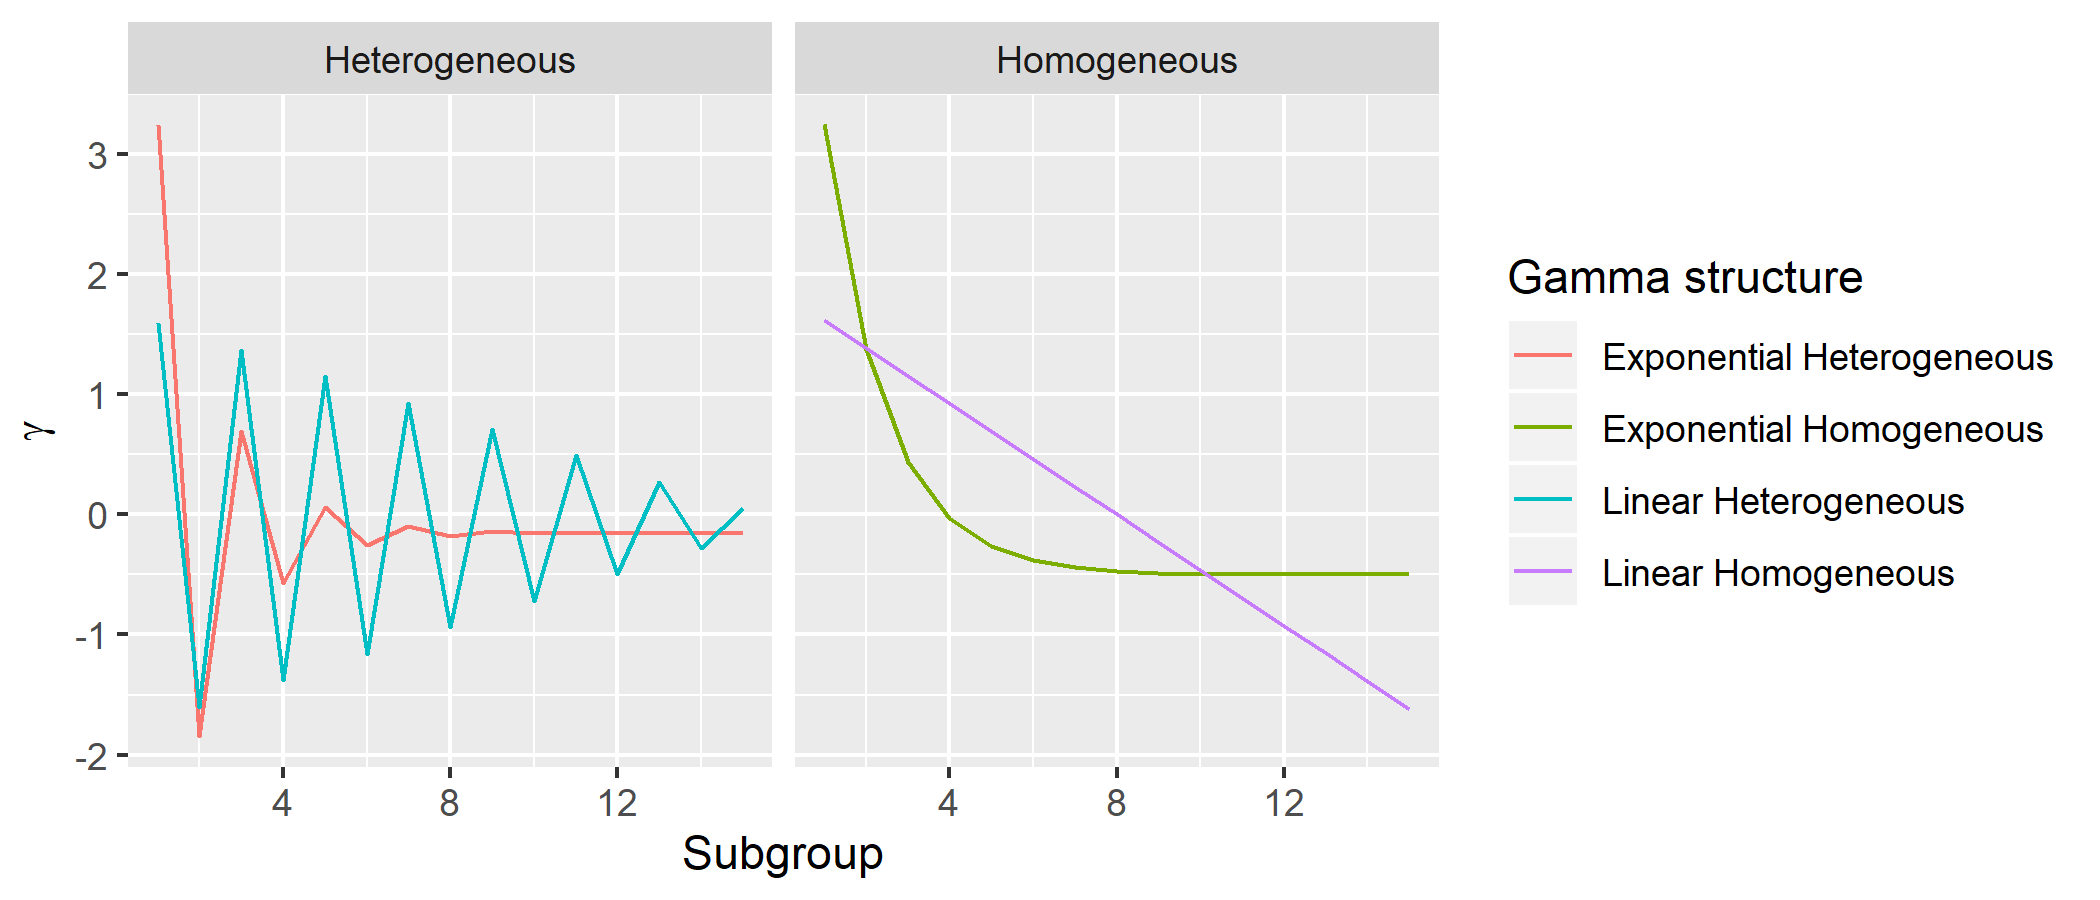
\includegraphics[scale = 0.9]{figures/gamma_structure.png}
    \caption{$\bgamma$ structures}
    \label{fig:gamma_structures}
\end{figure}



%%%%%%%%%%%%%%%%%%%%%%%%%%%%%%%%
%------------------------------%
%%%%%%%%%%%%%%%%%%%%%%%%%%%%%%%%
\section{Results} \label{sec:results}
%%%%%%%%%%%%%%%%%%%%%%%%%%%%%%%%
%------------------------------%
%%%%%%%%%%%%%%%%%%%%%%%%%%%%%%%%

%------------------------------%
\subsection{PC-Lasso and LMM-Lasso outperform Lasso in the presence of environmental confounding}
%------------------------------%

We begin by comparing the ordinary lasso, PC-Lasso, and LMM-Lasso as the level of environmental confounding is varied. Estimation accuracy for lasso, PC-Lasso, and LMM-Lasso was evaluated based on mean squared error (MSE) in various settings and broken down into bias and variance components.  Figure \ref{fig:mse} presents these results for all three data types in a 1:1 signal to noise (SNR) setting, where $\eta = 0.5$. The top row of figure \ref{fig:mse} shows that when $\xi = 0$ (i.e., no environmental confounding), lasso and LMM-Lasso perform comparably. PC-Lasso results in a slight inflation in MSE compared to the other methods due to the fact that 10 additional predictors have been added to the model, but none of them actually explain any variability in the outcome. The bottom row of figure \ref{fig:mse} shows the MSE when $\xi = 0.8$. In this case, both PC-Lasso and LMM-Lasso clearly outperform the naive lasso. This improvement is more substantial in the independent subpopulations simulated data than the admixed simulated data. This is due to the fact that the discrete, nonoverlapping genetic subpopulations more directly correspond to the distinct fixed environmental effects than do the more continuous and blended subpopulations in the admixture data.

\begin{figure}[H]
    \centering
    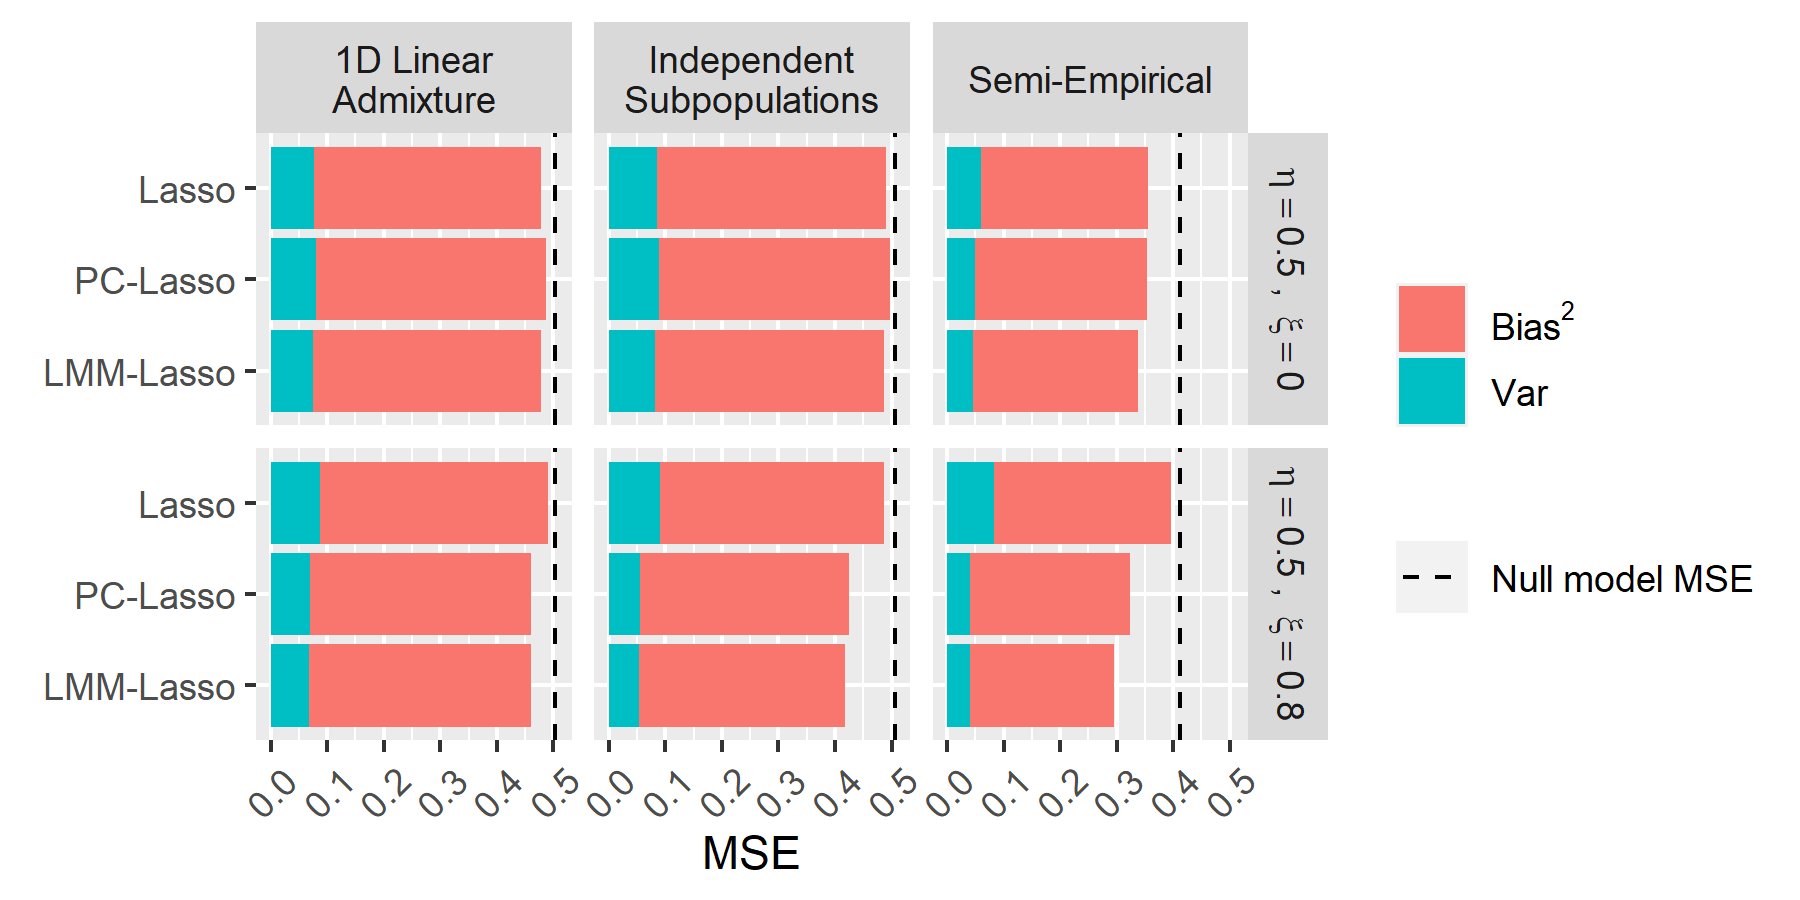
\includegraphics[scale = 1.1]{figures/beta_mse.png}
    \caption{Estimation accuracy of different methods for different data types in the presence and absence of environmental confounding with coarse subpopulation structure and dichotomous-\anna{heterogeneous/trans} environmental effects.}
    \label{fig:mse}
\end{figure}

\pb{Just FYI, it's hard to tell bias and var apart in black and white} \anna{will fix this, greek letters, labels}

%------------------------------%
\subsection{LMM-Lasso outperforms PC-Lasso when simulated subpopulations are small}
%------------------------------%

Given the superior performance of PC-Lasso and LMM-Lasso compared to the naive lasso in the presence of environmental confounding, we next compared these methods in the presence of fine and coarse subpopulation structures. 

Phenotypes were simulated using a 1:1 SNR, $\eta = 0.5$, and varying environmental confounding, $\xi \in \{0, 0.2, 0.5,0.8\}$. Figure \ref{fig:big_vs_small} summarizes the results of these simulations for the independent subpopulation simulated $\bX$ with environmental confounding simulated using a dichotomous-heterogeneous $\bgamma$ structure, though qualitatively similar results were observed for the other data types and $\gamma$ structures.

with the y-axis displaying the difference in MSE (PC-Lasso - LMM-Lasso) for each simulation and for the various subpopulation structures. The dashed horizontal line at 0 indicates no difference in the performance of PC-Lasso and LMM-Lasso, while differences greater than 0 correspond to smaller MSE for LMM-Lasso, and thus superior estimation accuracy. In the presence of a small number of large subpopulations, there is some overlap in the estimation accuracy of PC-Lasso and LMM-Lasso, as evidenced by the corresponding box straddling the 0 line. However, the majority of the box falls below 0, indicating the superior performance of PC-Lasso in many of the simulations. In the presence of many small subpopulations, however, LMM-Lasso is clearly superior to PC-Lasso in estimation accuracy. This is consistent with \citep{hoffman2013correcting}, who showed that principal component adjustment methods represent a low dimensional approximation to linear mixed models. As such, it is reasonable that PC-Lasso, which corrects for population structure using a low dimensional set of surrogate variables, would perform well in the small-number-of-large-subpopulations setting, but fall short in the presence of many small subpopulations. 
\begin{figure}[H]
    \centering
    % 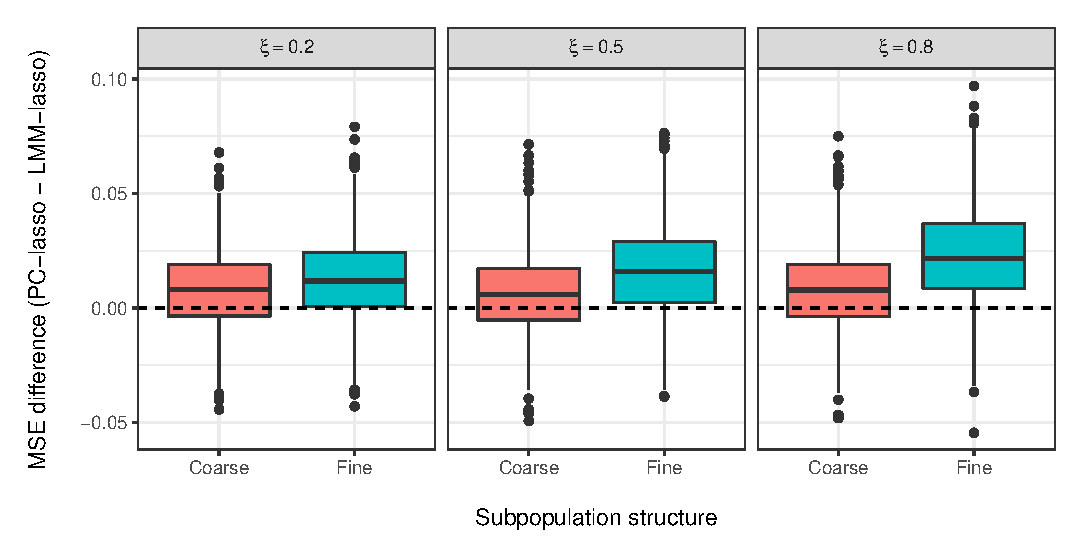
\includegraphics[scale = 0.9]{figures/mse_diff_subpops}
     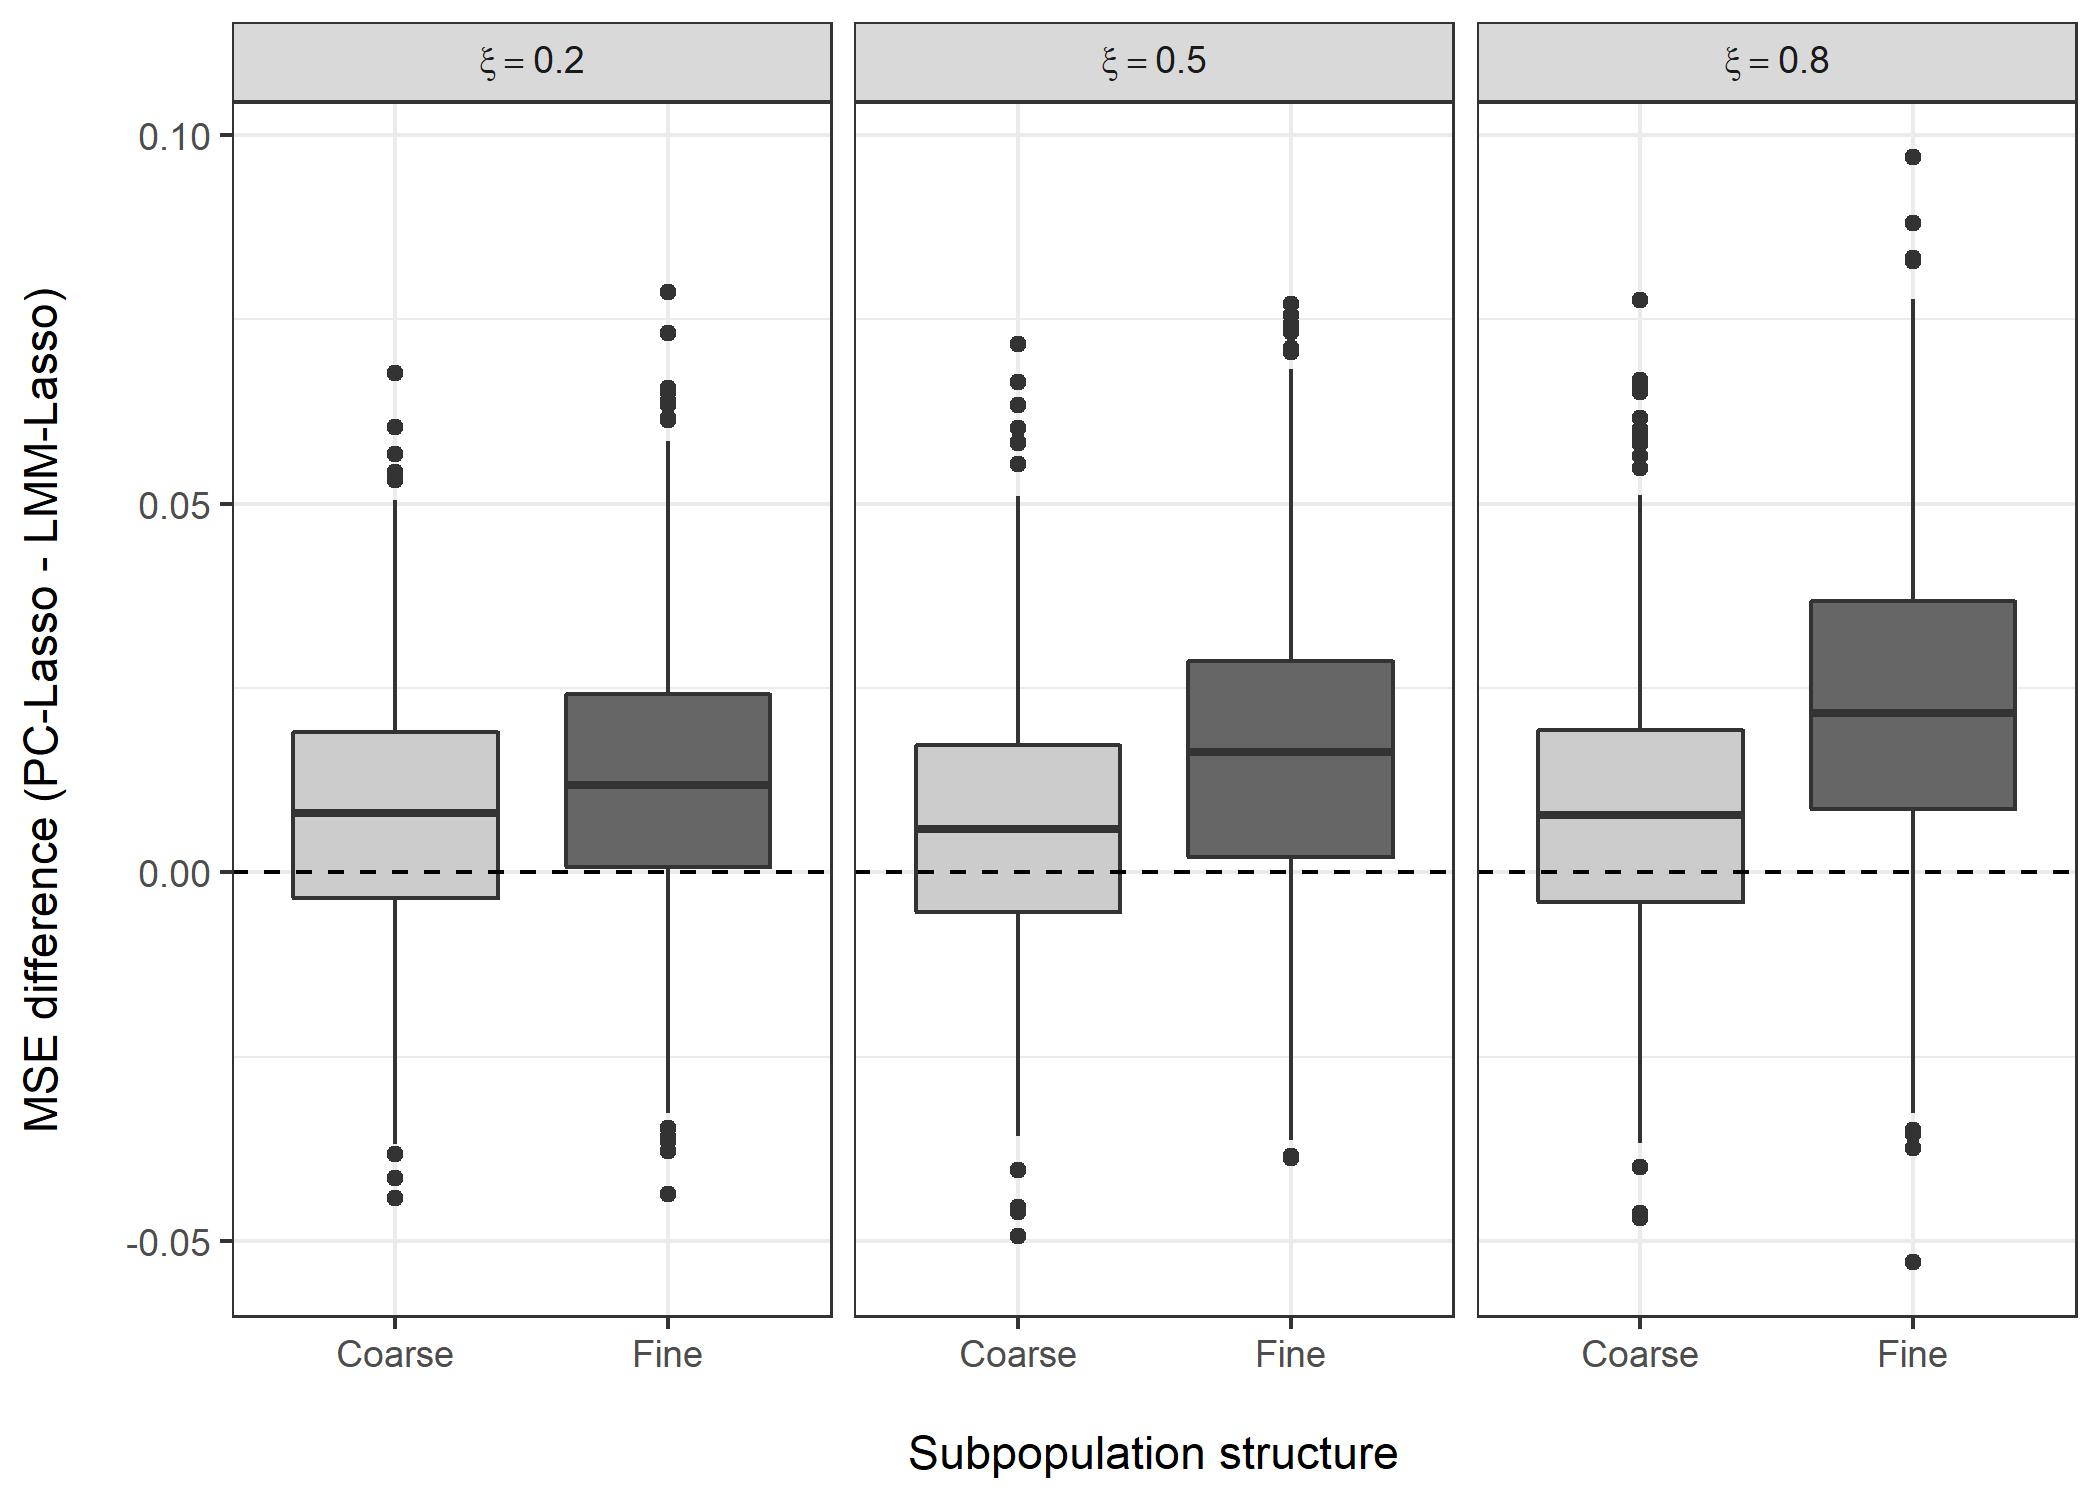
\includegraphics[scale = 0.9]{figures/mse_diff_subpops.png}
    \caption{Relative performance of LMM-Lasso, PC-Lasso for fine and coarse subpopulation structures and varying levels of environmental confounding with independent subpopulation data, $\eta = 0.5$, and dichotomous-\anna{heterogeneous/trans} environmental effects.}
    \label{fig:big_vs_small}
\end{figure}


%------------------------------%
\subsection{LMM-Lasso outperforms PC-Lasso when $\gamma$ is heterogeneous}
%------------------------------%

We evaluate PC-Lasso and LMM-Lasso in the presence of large and small subpopulations as well as distinct coefficient structures. Figure \ref{fig:big_small_gamma} shows the difference in MSE (PC-Lasso - LMM-Lasso) for all simulations, broken down by both subpopulation and coefficient structure. The right-hand panels of \ref{fig:big_small_gamma} are consistent with figure \ref{fig:big_vs_small}, showing superior LMM-Lasso performance in the presence of small subpopulations, regardless of coefficient linearity or homogeneity. The panel of figure \ref{fig:big_small_gamma} corresponding to large subpopulations with heterogeneous coefficients also appears to be a setting where LMM-Lasso consistently outperforms PC-Lasso, regardless of coefficient linearity. Only in the setting of large supopulations with homogeneous coefficients does PC-Lasso outperform LMM-Lasso. In line with our initial intuition, PC-Lasso performs best within this setting when coefficients are linear in nature. 

\begin{figure}[H]
    \centering
    % 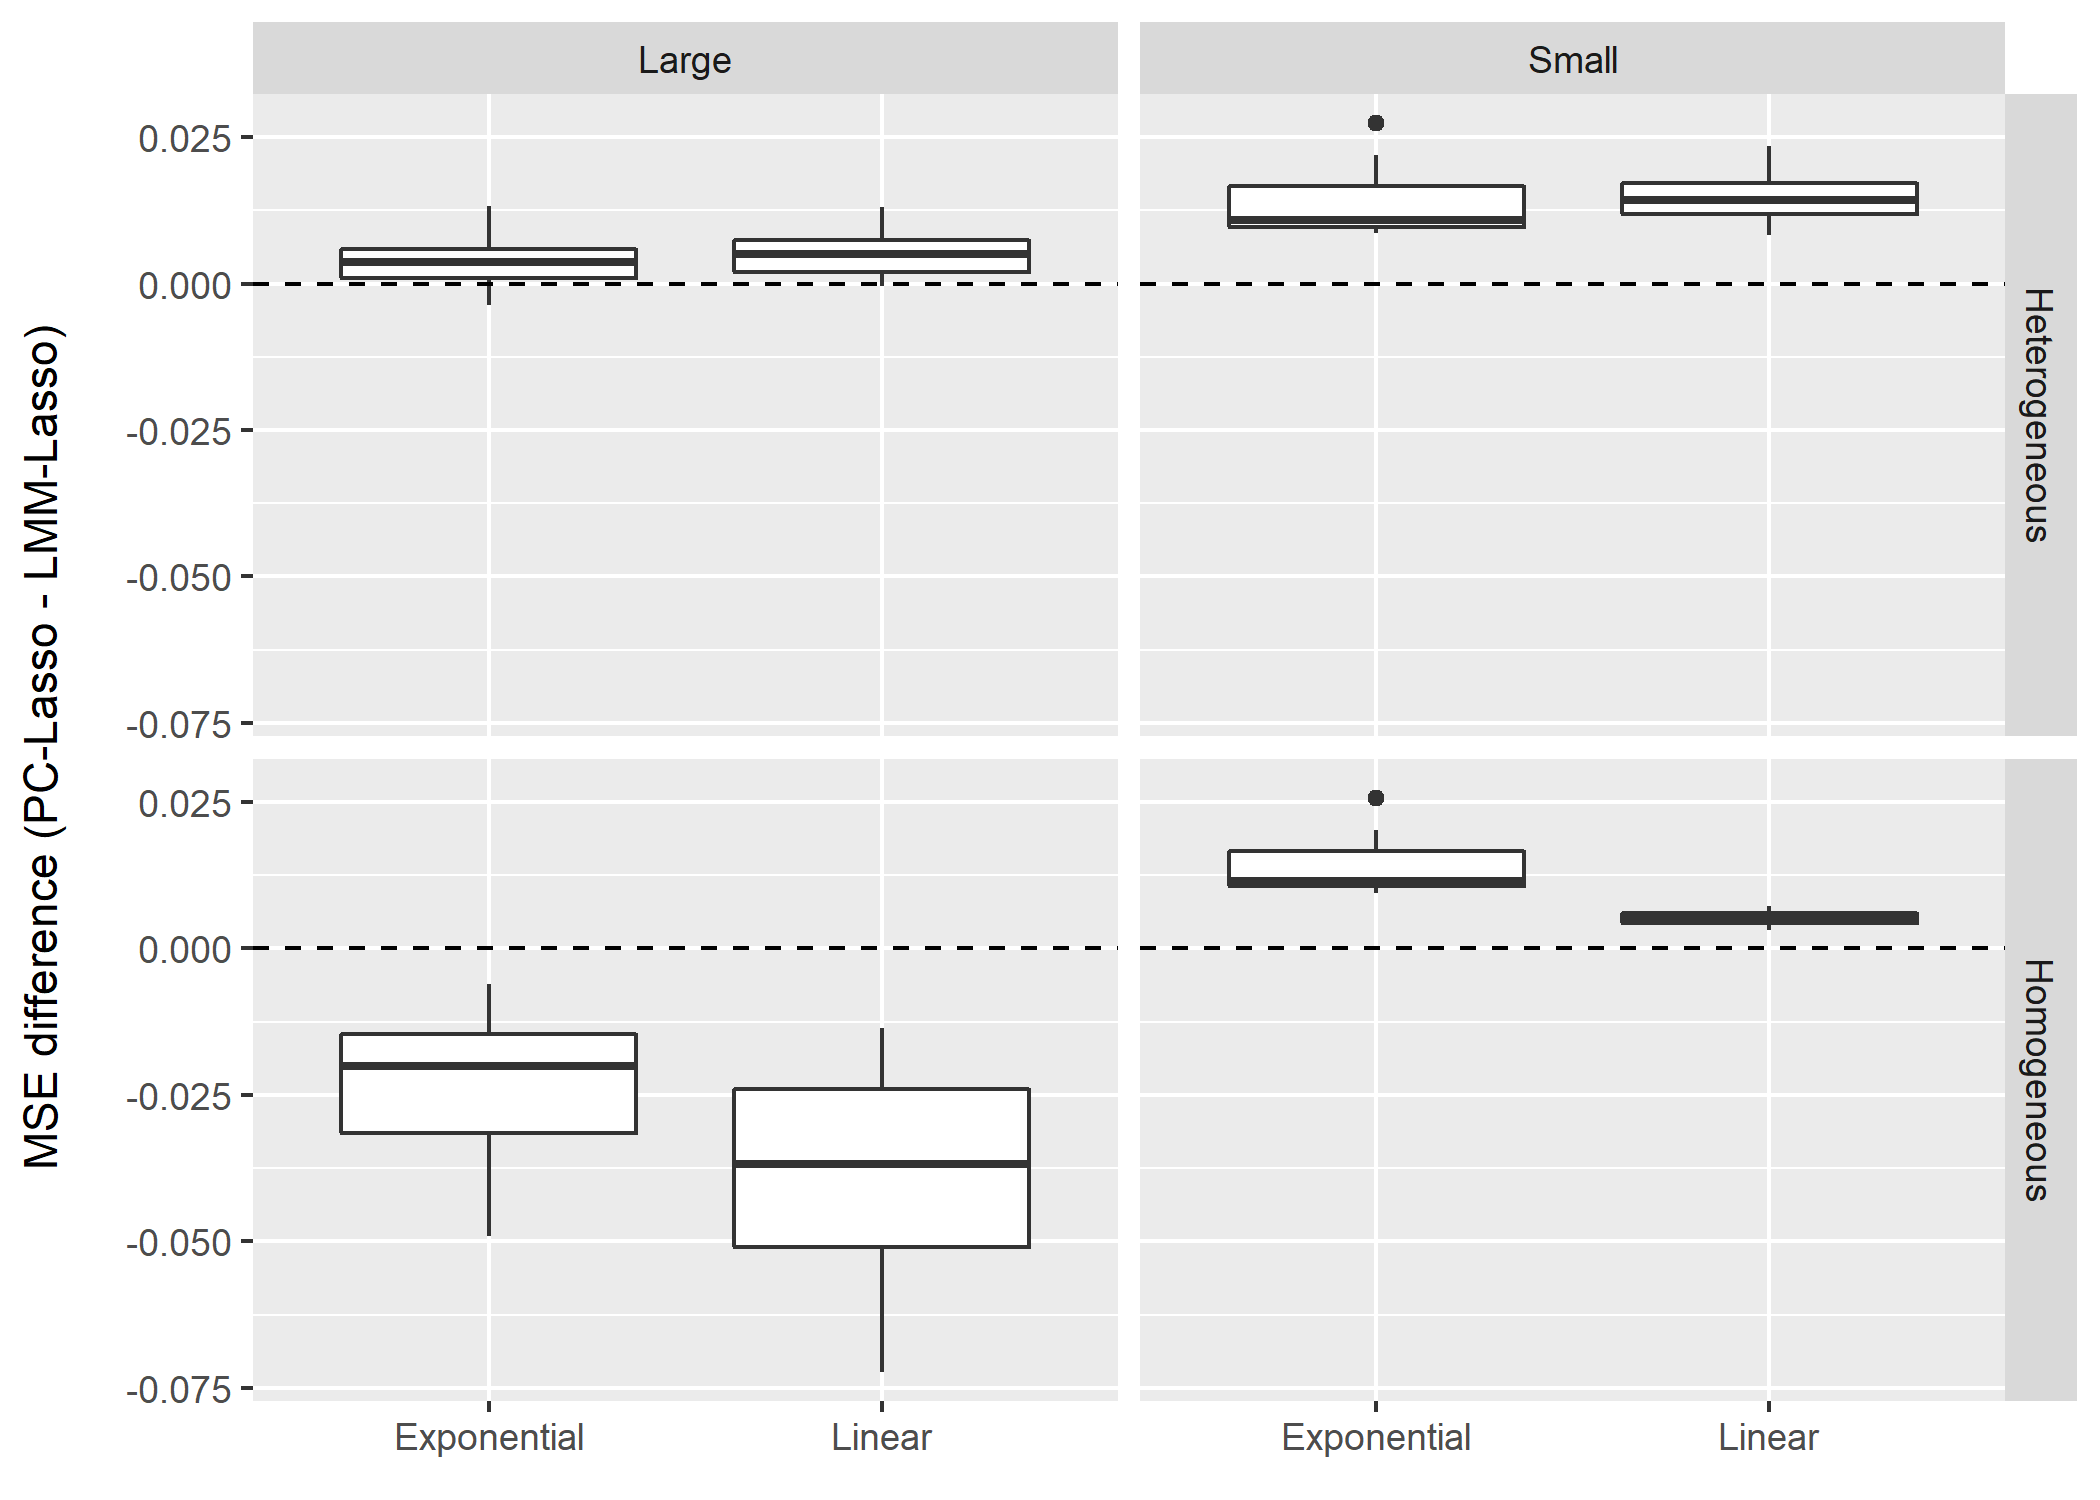
\includegraphics[scale = 0.9]{figures/fig2b.png}
    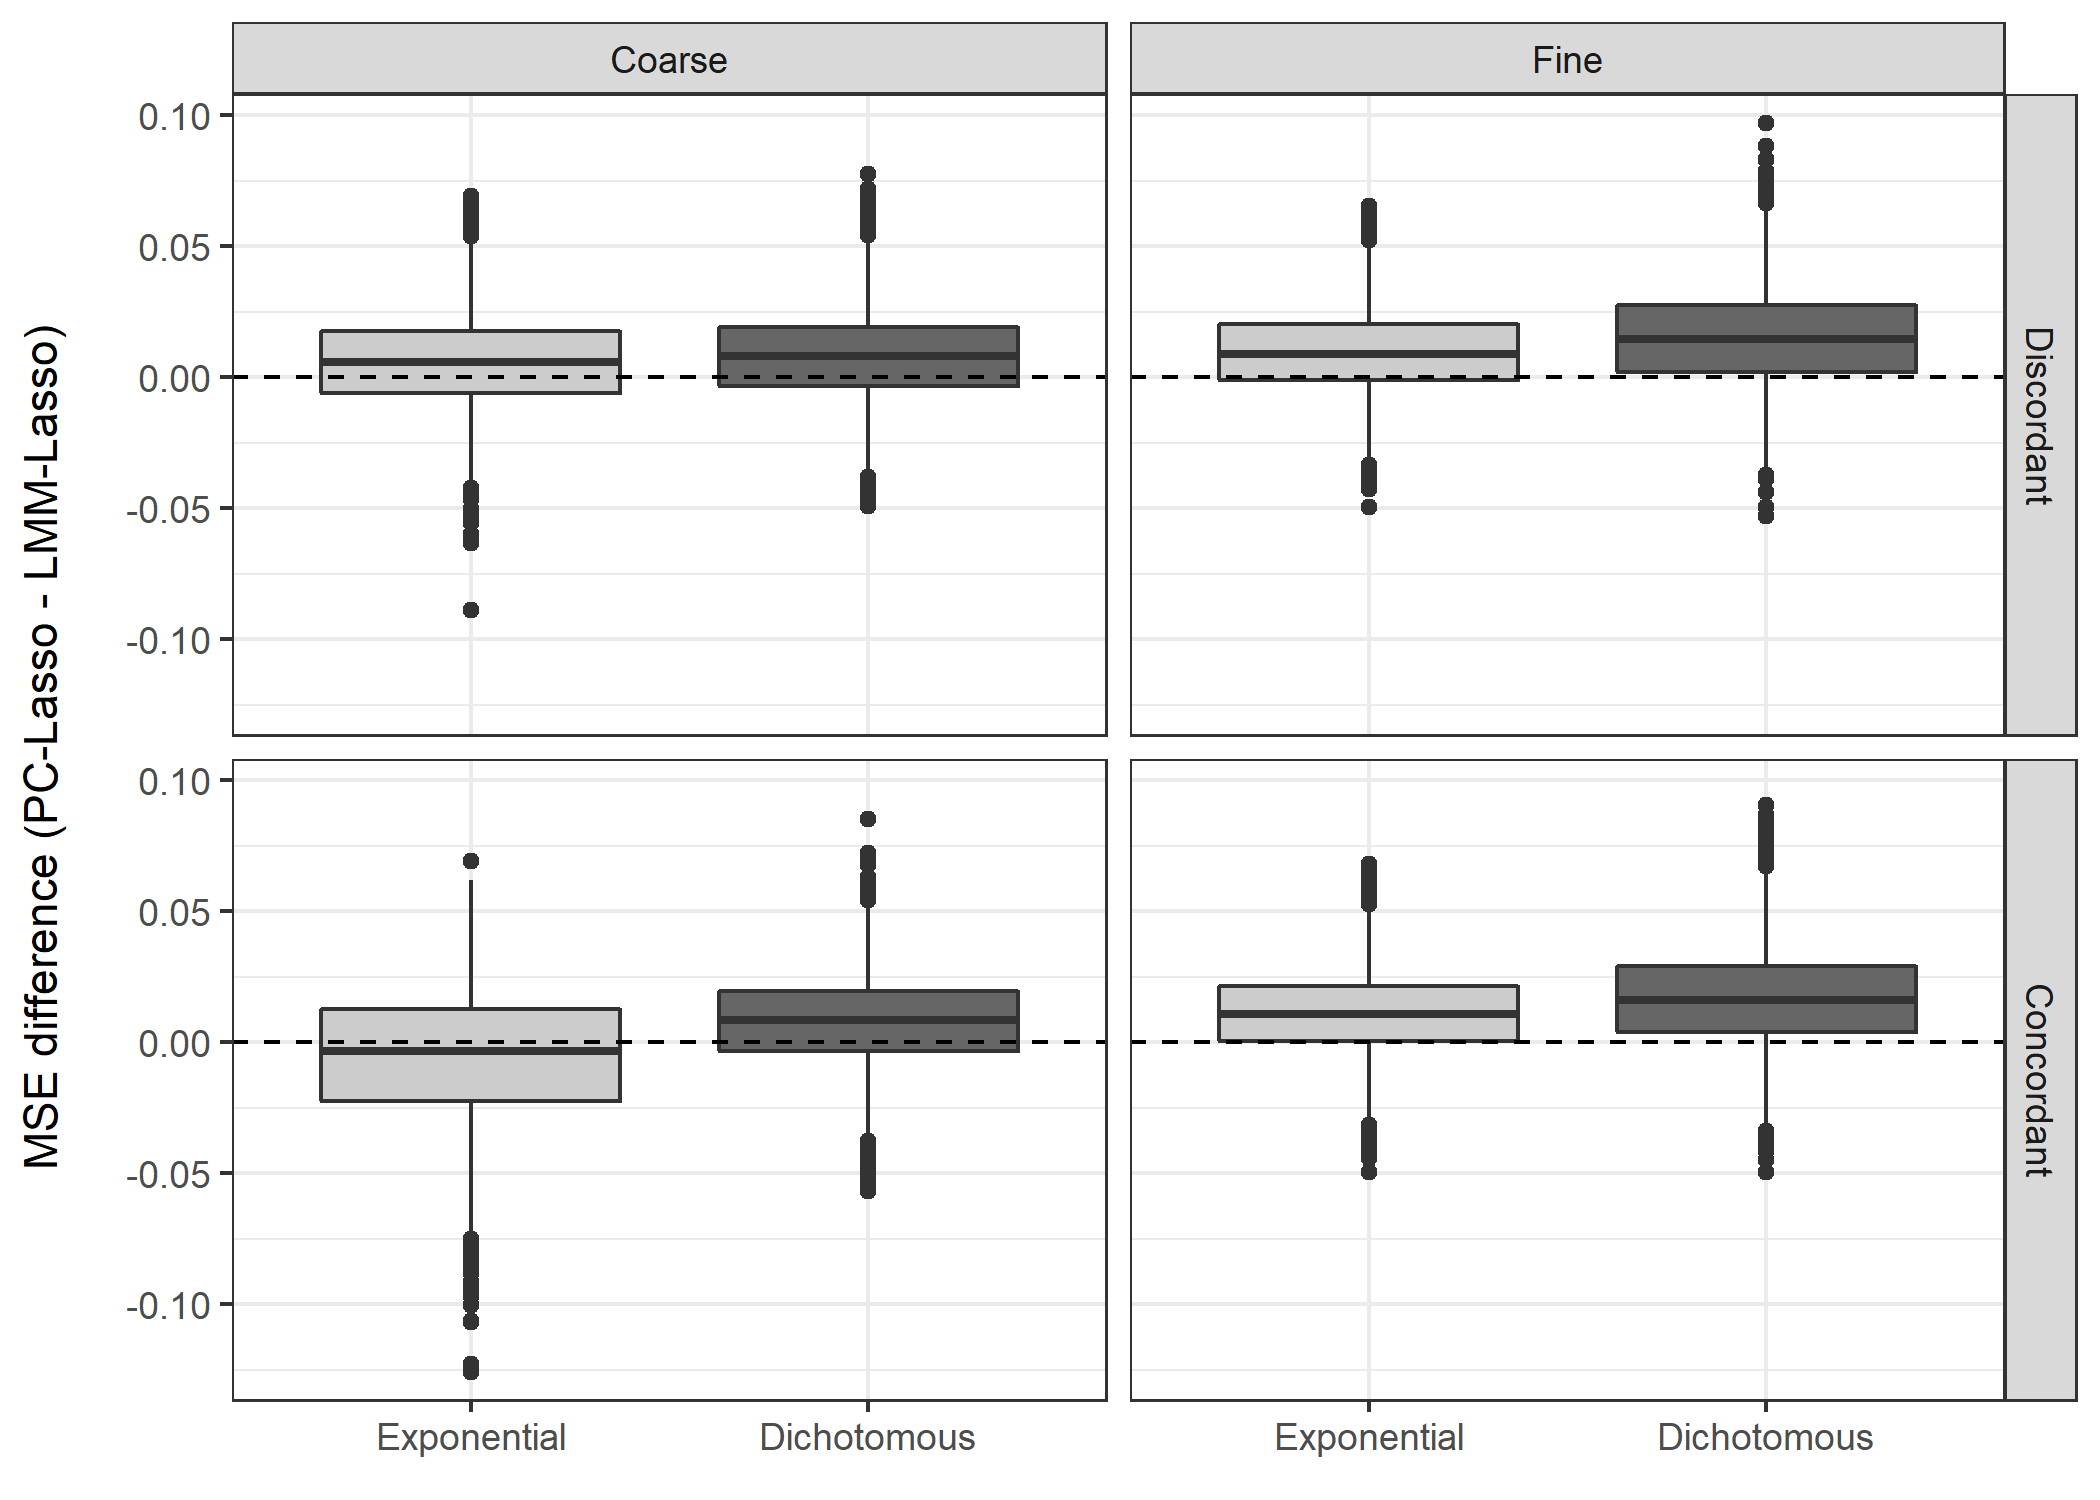
\includegraphics[scale = 0.9]{figures/mse_diff_hetero.png}
    \caption{Relative performance of LMM-Lasso, PC-Lasso for fine and coarse subpopulation structures and varying environmental effect structures with independent subpopulation data, $\eta = 0.5$, and $\xi = 0.8$}
    \label{fig:big_small_gamma}
\end{figure}

%------------------------------%
\subsection{Different implementations of LMM-Lasso}
%------------------------------%

Section~\ref{sec:rak-ggmix} briefly mentioned the existence of two LMM-Lasso variants: LMM-Lasso-Rakitsch and LMM-Lasso-ggmix. As we will see, the two generally perform quite similarly. Thus, the preceding results, although based on the LMM-Lasso-Rakitsch implementation, are representative of either LMM-Lasso method.

The primary purpose of this review is to compare LMM-Lasso to other penalized regression methods with respect to correcting for population structure and environmental confounding. However, given the generally strong performance of LMM-Lasso, we also wish to briefly discuss the key differences between these two ways of implementing it, and provide guidance for potential users.

LMM-Lasso-Rakitsch estimates the variance components once, under the assumption of a null model. LMM-Lasso-ggmix seeks to improve upon this by re-estimating the variance components and $\bbeta$ iteratively. Although this seems a reasonable approach, we have been unable to find a scenario where LMM-Lasso-ggmix outperforms the LMM-Lasso-Rakitsch in estimation accuracy of $\bbeta$ or $\eta$. 

\begin{figure}[H]
    \centering
    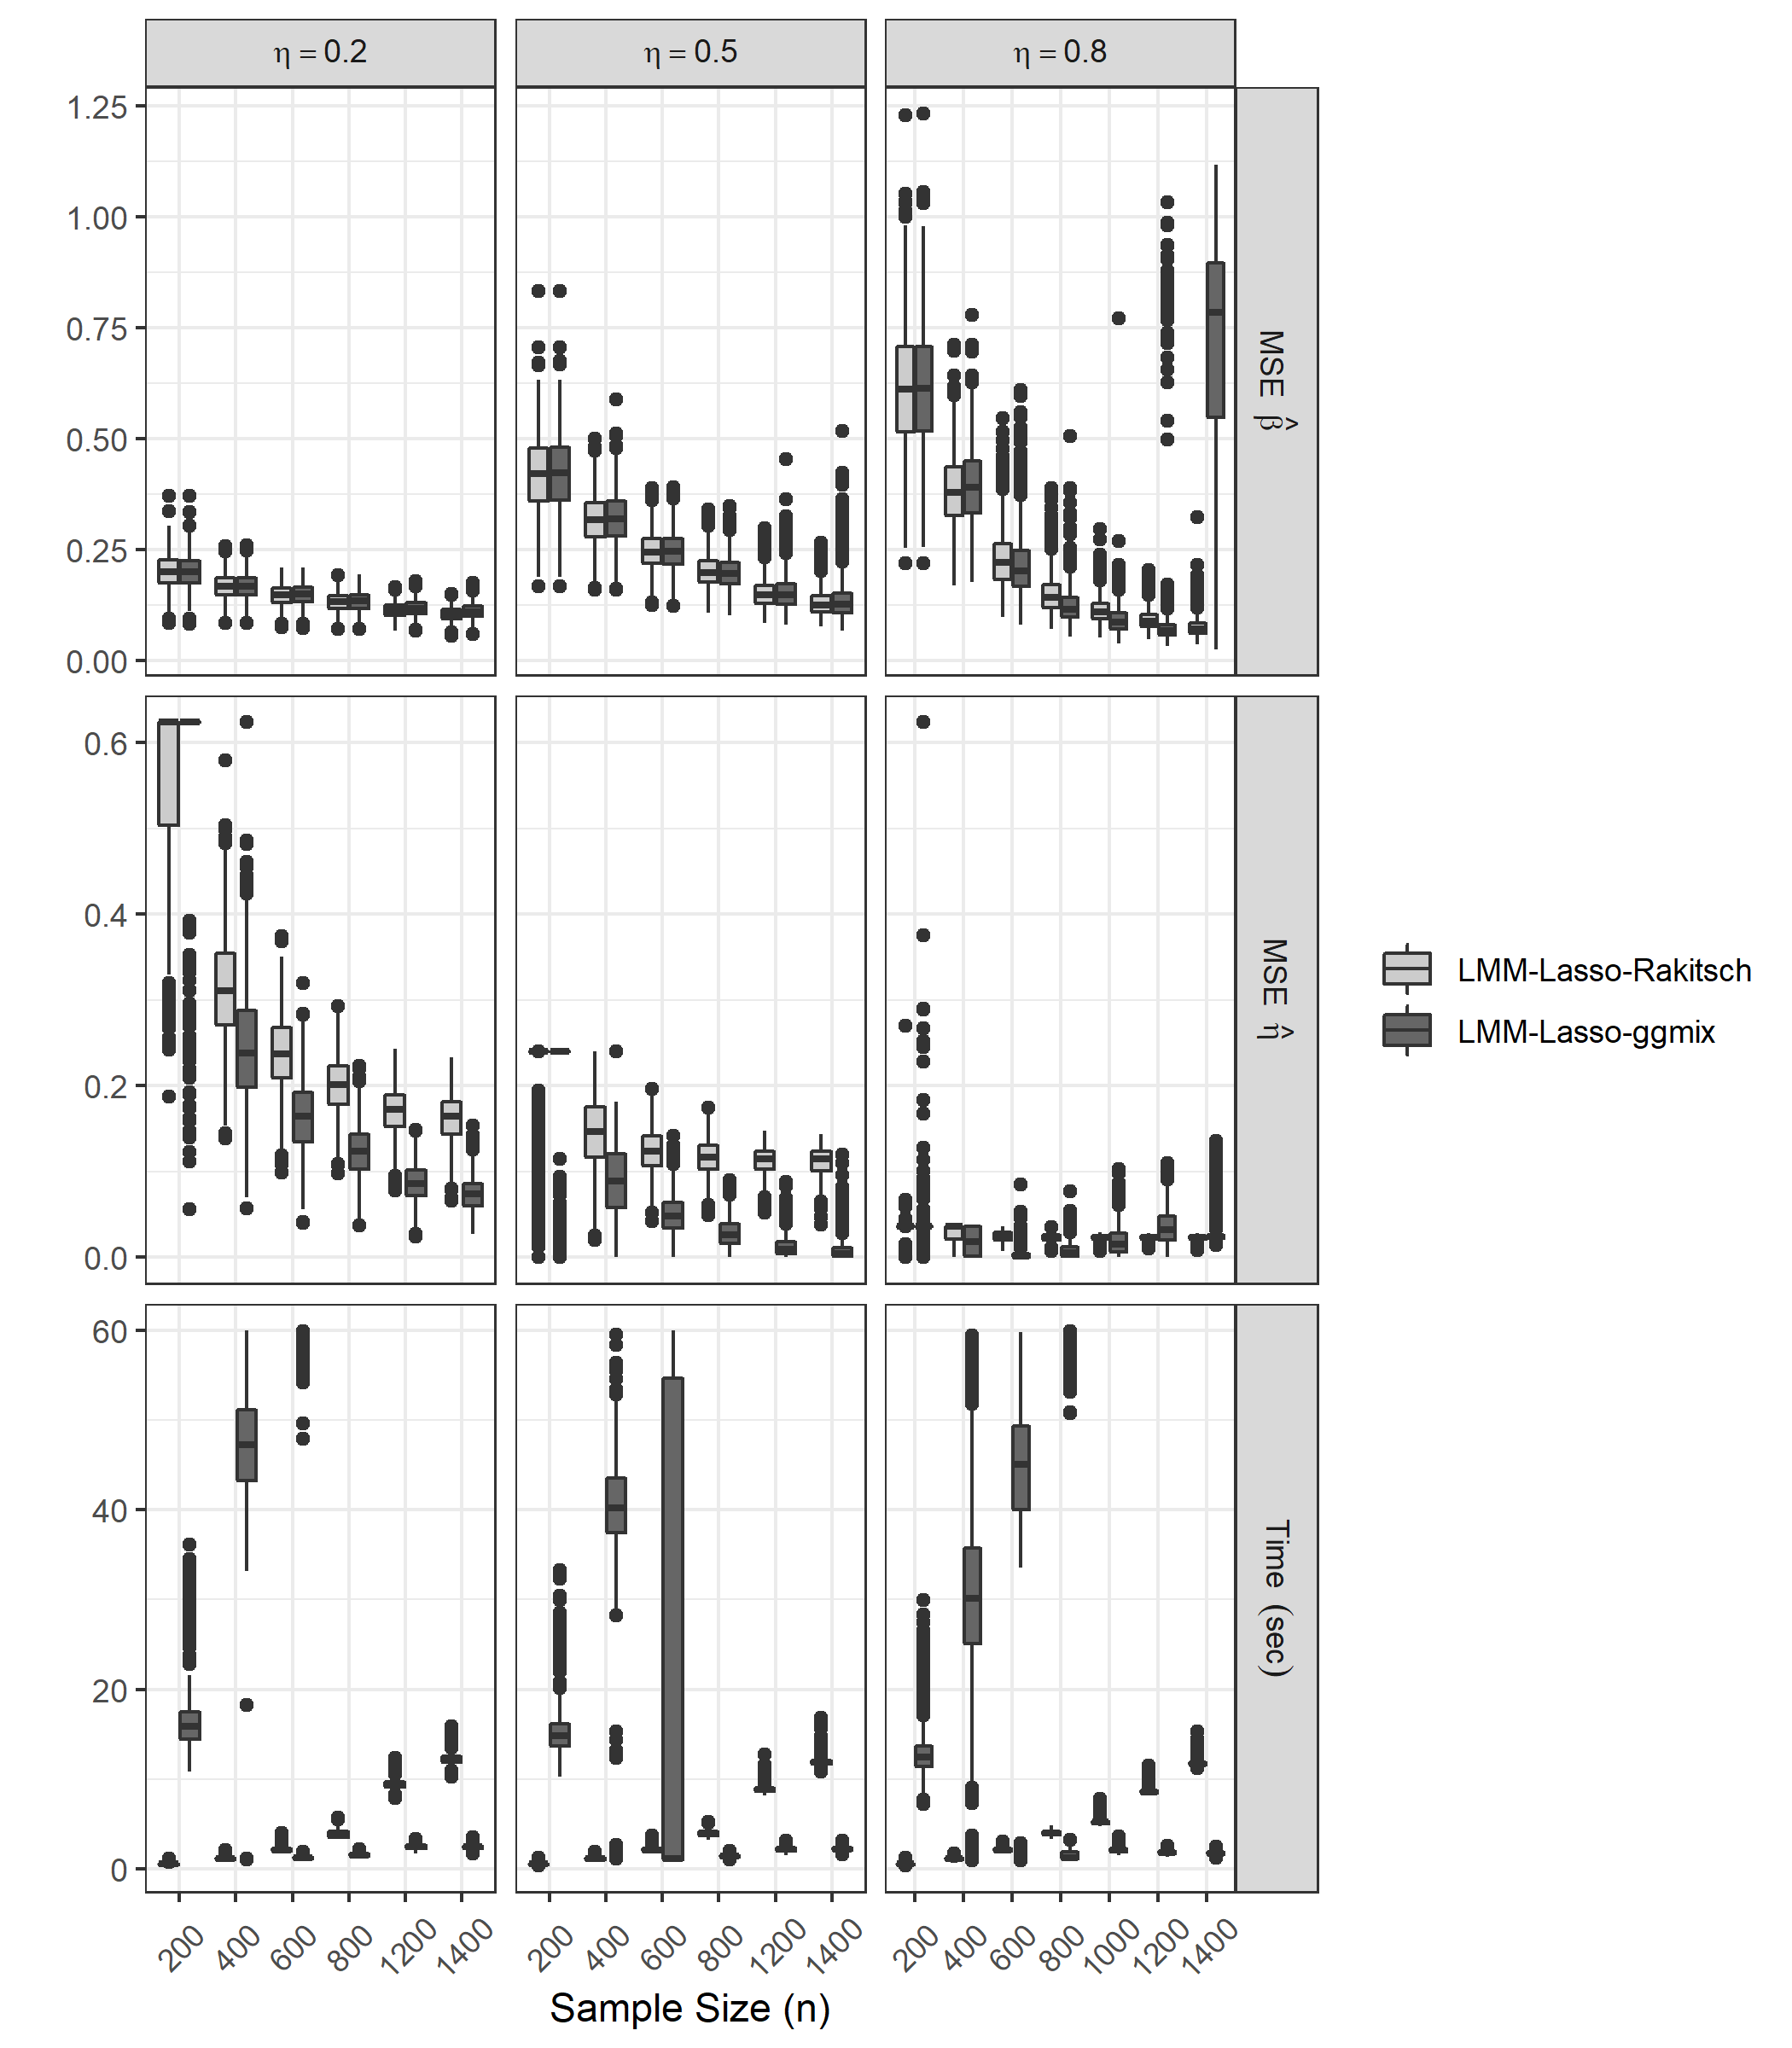
\includegraphics[scale = 1]{figures/eta_beta_hat.png}
     \caption{$\bbeta$ and $\eta$ estimation accuracy of LMM-Lasso-Rakitsch and LMM-Lasso-ggmix for varying $\eta$ levels and sample sizes with independent subpopulation data, coarse subpopulation structure, $\xi = 0.8$, and dichotomous-\anna{heterogeneous/trans} environmental effect structure.}
    \label{fig:eta_beta_mse}
\end{figure}


\begin{figure}[H]
    \centering
    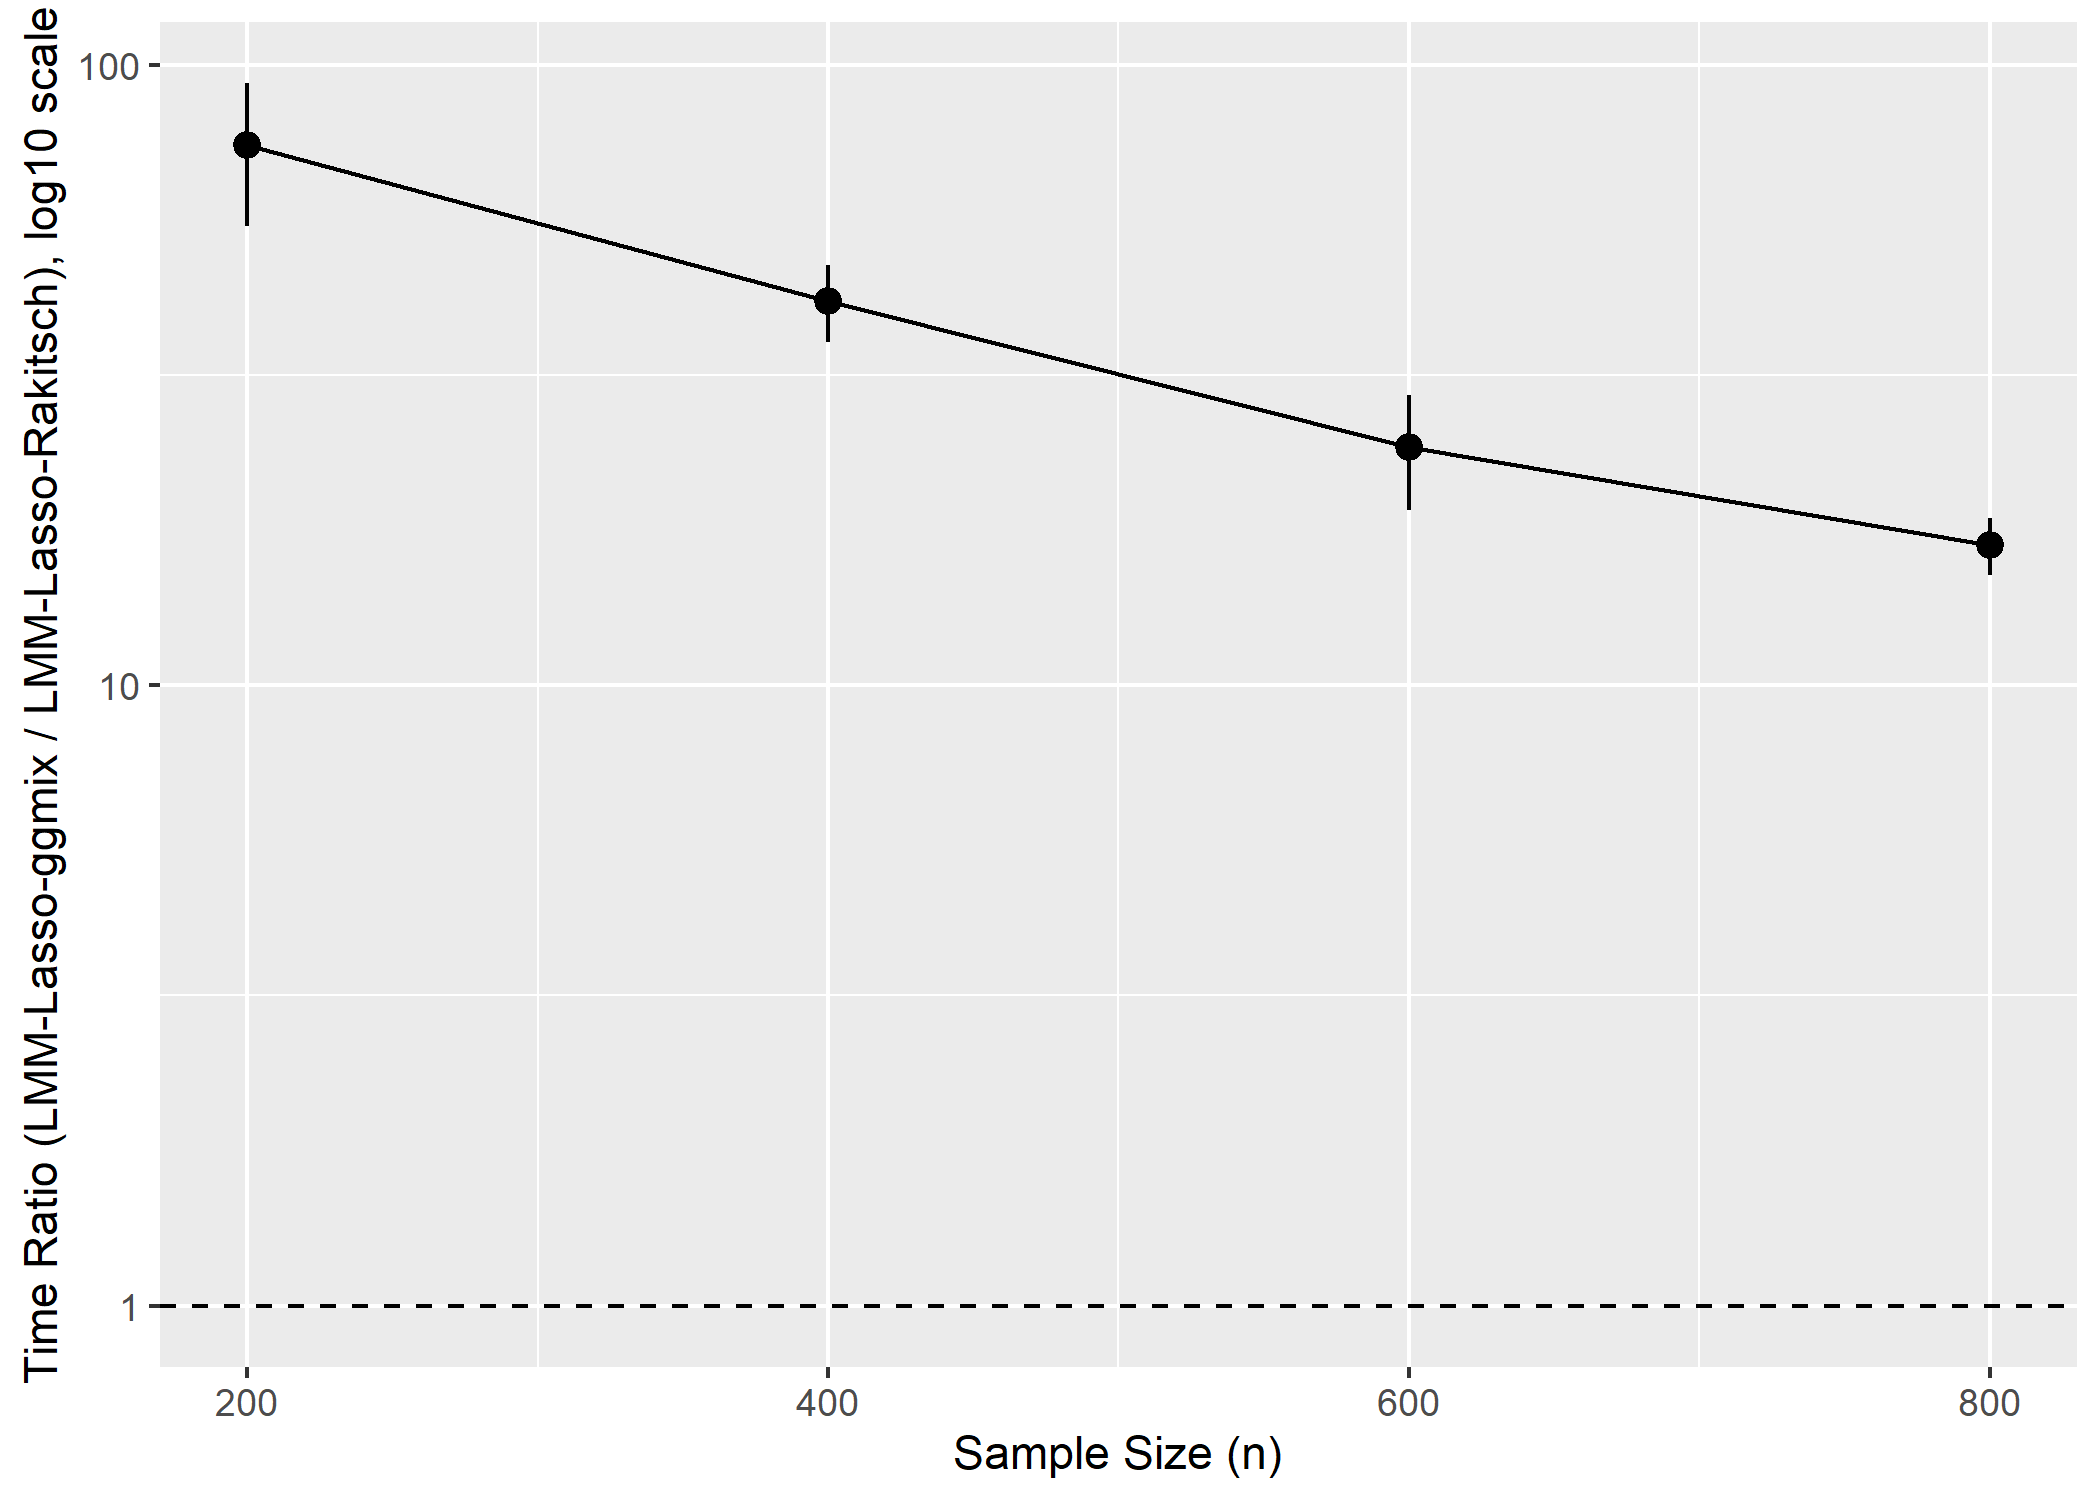
\includegraphics[scale = 0.8]{figures/time_ratio.png}
    \caption{Computing time of LMM-Lasso-Rakitsch compared with that of LMM-Lasso-ggmix for varying sample sizes with independent subpopulation structure, coarse subpopulation structure, $\eta = 0.5$, $\xi = 0.8$, and dichotomous-\anna{heterogeneous/trans} environmental effect structure.}
    \label{fig:time}
\end{figure}


In addition, we have found that LMM-Lasso-ggmix performs poorly in a low-dimensional setting due to the ill-conditioning of the RRM. Given its intended use for the analysis of high-dimensional data, this fact could be of little consequence to practitioners. However, although its estimation accuracy in high dimensions is on par with that of LMM-Lasso-Rakitsch, as shown in figure \ref{fig:eta_beta_mse}, this is also a setting in which the computational time required may be prohibitive for practical applications. Figure \ref{fig:time} shows the ratio of computing time required for LMM-Lasso-ggmix compared to that of LMM-Lasso-Rakitsch, for various sample sizes. The horizontal dashed line at 1 indicates both methods require the same computing time. Despite its comparable performance in accurately estimating $\hat{\bbeta}$, LMM-Lasso-ggmix takes approximately 71 to 9 times as long as LMM-Lasso-Rakitsch. Thus, LMM-Lasso-Rakitsch seems to be a more attractive and scalable method than LMM-Lasso-ggmix.


%%%%%%%%%%%%%%%%%%%%%%%%%%%%%%%%
%------------------------------%
%%%%%%%%%%%%%%%%%%%%%%%%%%%%%%%%
\section{Discussion} \label{sec:discussion}
%%%%%%%%%%%%%%%%%%%%%%%%%%%%%%%%
%------------------------------%
%%%%%%%%%%%%%%%%%%%%%%%%%%%%%%%%
In this work, we have reviewed the concept of population stratification and defined explicitly the environmental (i.e., non-genetic) mechanism by which it may confound the genotype-phenotype relationship. We have provided a broad outline of existing methods for ameliorating the effects of these unobserved confounding influences. In addition, we have provided a thorough review of two popular approaches for correcting for population structure in genetic data: PC-Lasso and LMM-Lasso. 

We have detailed the assumptions made by PC-Lasso and LMM-Lasso, which model confounding influences as fixed and random effects, respectively. We have also detailed the ways in which simulation schemes to evaluate these methods may fail to accurately capture the effects of environmental heterogeneity. In turn, we propose and utilize a simulation approach in which the estimation bias introduced by environmental heterogeneity may be evaluated. We then compare the estimation accuracy of a naive lasso, PC-Lasso, and LMM-Lasso in various confounding scenarios.

Unsurprisingly, we find that PC-Lasso and LMM-Lasso outperform the naive lasso whenever environmental confounding effects are present. However, in the absence of such effects, PC-Lasso may hinder estimation accuracy and perform more poorly than even the naive lasso. This is due to the fact that the principal components are unpenalized and thus included in the final model, even when they do more harm than good in explaining phenotypic variability. Additionally, we find that LMM-Lasso outperforms PC-Lasso when (1) small genetic subpopulations are present which correspond to environmental heterogeneity and (2) when confounding effects are nonlinear and heterogeneous in nature. In the presence of large subpopulations which correspond to homogeneous, linear environmental effects, PC-Lasso and LMM-Lasso perform comparably in estimation accuracy. While this scenario may be plausible, given that LMM-Lasso is more robust to subpopulation sizes and nonlinear effects, it may present a 'safer choice' for practitioners seeking to obtain unbiased estimates when the exact nature of population structure and corresponding environmental heterogeneity are unknown.  

We considered two implementations of the LMM-Lasso method: LMM-Lasso-Rakitsch and LMM-Lasso-ggmix, which differ in their variance estimation procedures and computational implementations. Although we found that both methods perform similarly in terms of estimation accuracy in many scenarios, LMM-Lasso-ggmix has several distinct disadvantages. Firstly, it suffers from instability in low dimensions. Secondly, although LMM-Lasso-Rakitsch and LMM-Lasso-ggmix perform comparably in high dimensions, LMM-Lasso-ggmix takes approximately \anna{x} times longer due to its iterative estimation procedure. Thirdly, while the additional time required of LMM-Lasso-ggmix could be worthwhile if it resulted in a more accurate estimation of $\eta$, or narrow-sense heritability, we have been unable to identify a scenario where its narrow-sense heritability estimates are superior to those of LMM-Lasso-Rakitsch. We have implemented the LMM-Lasso-Rakitsch method using the equivalent but more interpretable $\eta$ paramaterization in the \texttt{R} package, \texttt{penalizedLMM (final name tbd)}, available on the author's github page: \url{https://github.com/areisett/penalizedLMM}.

\pb{Introduce penalizedLMM here, or in next paper?}

Even in scenarios where LMM-Lasso outperforms other methods, its estimation accuracy still suffers due to the bias inherent in penalized regression methods. Because of this, bias-reduction techniques for penalized LMMs may be an attractive avenue for future research.

